%===============================================================================
% LaTeX sjabloon voor de bachelorproef toegepaste informatica aan HOGENT
% Meer info op https://github.com/HoGentTIN/latex-hogent-report
%===============================================================================

\documentclass[english,dit,thesis]{hogentreport}

% - If necessary, replace the option `dit`' with your own department!
%   Valid entries are dbo, dbt, dgz, dit, dlo, dog, dsa, soa
% - If you write your thesis in English (remark: only possible after getting
%   explicit approval!), remove the option "dutch," or replace with "english".

\usepackage{lipsum} % For blind text, can be removed after adding actual content
\usepackage[table]{xcolor}% http://ctan.org/pkg/xcolor


%% Pictures to include in the text can be put in the graphics/ folder
\graphicspath{{../graphics/}}

%% For source code highlighting, requires pygments to be installed
%% Compile with the -shell-escape flag!
\usepackage[chapter]{minted}
%% If you compile with the make_thesis.{bat,sh} script, use the following
%% import instead:
%%\usepackage[chapter,outputdir=../output]{minted}
%%\usemintedstyle{solarized-light}

%% Formatting for minted environments.
\setminted{%
    autogobble,
    frame=lines,
    breaklines,
    linenos,
    tabsize=4
}

\emergencystretch=1em

%% Ensure the list of listings is in the table of contents
\renewcommand\listoflistingscaption{%
    \IfLanguageName{dutch}{Lijst van codefragmenten}{List of listings}
}
\renewcommand\listingscaption{%
    \IfLanguageName{dutch}{Codefragment}{Listing}
}
\renewcommand*\listoflistings{%
    \cleardoublepage\phantomsection\addcontentsline{toc}{chapter}{\listoflistingscaption}%
    \listof{listing}{\listoflistingscaption}%
}

% Other packages not already included can be imported here

%%---------- Document metadata -------------------------------------------------
% TODO: Replace this with your own information
\author{Mike De Decker}
\supervisor{Ms. L. De Mol}
\cosupervisor{Mr. D. Plummer}
\title{\IfLanguageName{dutch}{AI jury-assistent voor het herkennen van rope skipping skills in videos}{AI judge for recognition of jump rope skills in videos}}
\academicyear{\advance\year by -1 \the\year--\advance\year by 1 \the\year}
\examperiod{2}
\degreesought{\IfLanguageName{dutch}{Professionele bachelor in de toegepaste informatica}{Bachelor of applied computer science}}
\partialthesis{false} %% To display 'in partial fulfilment'
%\institution{Internshipcompany BVBA.}

%% Add global exceptions to the hyphenation here
\hyphenation{back-slash}

%% The bibliography (style and settings are  found in hogentthesis.cls)
\addbibresource{bachproef.bib}            %% Bibliography file
\addbibresource{../voorstel/voorstel.bib} %% Bibliography research proposal
\defbibheading{bibempty}{}

%% Prevent empty pages for right-handed chapter starts in twoside mode
\renewcommand{\cleardoublepage}{\clearpage}

\renewcommand{\arraystretch}{1.2}

%% Content starts here.
\begin{document}

%---------- Front matter -------------------------------------------------------

\frontmatter

\hypersetup{pageanchor=false} %% Disable page numbering references
%% Render a Dutch outer title page if the main language is English
\IfLanguageName{english}{%
    %% If necessary, information can be changed here
    \degreesought{Professionele Bachelor toegepaste informatica}%
    \begin{otherlanguage}{dutch}%
       \maketitle%
    \end{otherlanguage}%
}{}

%% Generates title page content
\maketitle
\hypersetup{pageanchor=true}

%%=============================================================================
%% Voorwoord
%%=============================================================================

\chapter*{\IfLanguageName{dutch}{Woord vooraf}{Preface}}%
\label{ch:voorwoord}

%% TODO:
%% Het voorwoord is het enige deel van de bachelorproef waar je vanuit je
%% eigen standpunt (``ik-vorm'') mag schrijven. Je kan hier bv. motiveren
%% waarom jij het onderwerp wil bespreken.
%% Vergeet ook niet te bedanken wie je geholpen/gesteund/... heeft

As a passionate jump roper, student of applied informatics, I came to the idea of creating an AI skill recognition system based on earlier seen ideas of sign langue detection and emotion recognition. These examples planted a blooming seed which I've proudly grown during my thesis.

I want to thank my promotors Lena De Mol and Thomas Parmentier for the feedback on the paper and the process.
I also want give a big thanks to my co-promotor Dylan Plummer, to aid this Belgian Machine Learning enthiousast into tips and tricks for computer vision, model exploration, concepts and so much more.
I also want to thank Pieter Gibens en Sara De Boever to aid in all my judging questions.
Another special mention is for Gymfed, Eva and Arne, allowing to use earlier competition recordings and for the permission to record freestyles myself from 'behind' the judging table.
I also want to thank Hogent (BIB Lera) for the ability to rent cameras.
During the thesis, I've had a lot of joy in extending my judging knowledge, coding, labeling, training models, inspecting results and creating the Vue3 web app displaying some statistics.

The thesis may have finished, but I've only just begun!
%%=============================================================================
%% Samenvatting
%%=============================================================================

% TODO: De "abstract" of samenvatting is een kernachtige (~ 1 blz. voor een
% thesis) synthese van het document.
%
% Een goede abstract biedt een kernachtig antwoord op volgende vragen:
%
% 1. Waarover gaat de bachelorproef?
% 2. Waarom heb je er over geschreven?
% 3. Hoe heb je het onderzoek uitgevoerd?
% 4. Wat waren de resultaten? Wat blijkt uit je onderzoek?
% 5. Wat betekenen je resultaten? Wat is de relevantie voor het werkveld?
%
% Daarom bestaat een abstract uit volgende componenten:
%
% - inleiding + kaderen thema
% - probleemstelling
% - (centrale) onderzoeksvraag
% - onderzoeksdoelstelling
% - methodologie
% - resultaten (beperk tot de belangrijkste, relevant voor de onderzoeksvraag)
% - conclusies, aanbevelingen, beperkingen
%
% LET OP! Een samenvatting is GEEN voorwoord!

%%---------- Nederlandse samenvatting -----------------------------------------
%
% TODO: Als je je bachelorproef in het Engels schrijft, moet je eerst een
% Nederlandse samenvatting invoegen. Haal daarvoor onderstaande code uit
% commentaar.
% Wie zijn bachelorproef in het Nederlands schrijft, kan dit negeren, de inhoud
% wordt niet in het document ingevoegd.

\IfLanguageName{english}{%
\selectlanguage{dutch}
\chapter*{Samenvatting}
\lipsum[1-4]
\selectlanguage{english}
}{}

%%---------- Samenvatting -----------------------------------------------------
% De samenvatting in de hoofdtaal van het document

\chapter*{\IfLanguageName{dutch}{Samenvatting}{Abstract}}

Judging jump rope freestyle routines at the highest competitive level has become increasingly challenging due to the evolution of jump rope. Both the number of skills that are included in a routine as well as the speed with which these are executed keep increasing. This is particularly evident in so-called Double Dutch Freestyle routines, which is why assigning scores to these freestyles is done by a combination of live and delayed evaluation. The creativity of a routine (including its variation and musicality) is scored in real time but the assignment of the appropriate difficulty level is done based on a recording of the routine replayed at half speed right after it is performed. Even though this helps reduce errors in difficulty scoring, a certain variability in the assigned scores persists/can still be seen. With the increased accessibility of artificial intelligence, particularly neural networks, the question arises whether an AI judge or assistant can be developed to obtain a more accurate (objective) difficulty scoring.

This research explores the possibility and development of such an AI assistant, as well as the techniques and challenges required to obtain the desired level of objectivity.
The current idea is divided into three sections. The first section will be localizing the jumpers in the field as most obtained recordings are not fully zoomed in or recorded using a static camera. As recorded jumpers sometimes take up less than a fifth of the recording, they can be cropped out sparing computational resources for the parts to come. The second part involves isolating skills from a routine into individual skills or subskills. This enables the assistant to not only label a single skill, but also dozens of skills performed sequentially without interference. Lastly, each segment can be assigned to its corresponding skill. For Double Dutch Freestyles this means the combined action of jumpers and turners resulting in a large possibility of unique combinations. By further marking presentational skills or difficult to see skills as unknown (e.g. when one athlete stands between others and the camera) it is expected that the AI judge will indicate unknown or unclear skills by itself. This way the the assistant can be put into practice when reaching similar or more accurate results than the live jury panel. The assistant's results allow for verification of scores during and after the competition, increasing transparency and accuracy even further. Using the current obtained competition videos displaying the most common skills a few hundred times, it is expected that the AI judge will start to distinguish between skills like a cartwheel, split or salto.
In case it works, it is not only useful for jump rope freestyles but also applicable in other judge-related competitions such as gymnastic routines, figure skating, or synchronized swimming.


%---------- Inhoud, lijst figuren, ... -----------------------------------------

\tableofcontents

% In a list of figures, the complete caption will be included. To prevent this,
% ALWAYS add a short description in the caption!
%
%  \caption[short description]{elaborate description}
%
% If you do, only the short description will be used in the list of figures

\listoffigures

% If you included tables and/or source code listings, uncomment the appropriate
% lines.
\listoftables

\listoflistings

% Als je een lijst van afkortingen of termen wil toevoegen, dan hoort die
% hier thuis. Gebruik bijvoorbeeld de ``glossaries'' package.
% https://www.overleaf.com/learn/latex/Glossaries

%---------- Kern ---------------------------------------------------------------

\mainmatter{}

% De eerste hoofdstukken van een bachelorproef zijn meestal een inleiding op
% het onderwerp, literatuurstudie en verantwoording methodologie.
% Aarzel niet om een meer beschrijvende titel aan deze hoofdstukken te geven of
% om bijvoorbeeld de inleiding en/of stand van zaken over meerdere hoofdstukken
% te verspreiden!

%%=============================================================================
%% Inleiding
%%=============================================================================

\chapter{\IfLanguageName{dutch}{Inleiding}{Introduction}}%
\label{ch:inleiding}

Jump rope is an evolving sport.
Year after year, an increasing amount of high-level competitors are pushing the limits of jump rope.
% TODO : source?
This results in new skills, new combinations, better physiques, better rope material, and faster movements. For the judges to keep up with the jumpers and to correctly assess scores to a routine, Double Dutch freestyles \footnote{Two turners, with one or more jumpers}, one of the jump rope disciplines, are reviewed at half speed in International competitions or even at nationals in Belgium.

Head judges around the world question the best way to judge athletes correctly so as to give an accurate and objective ranking in national or international competitions.
Many solutions have been provided: another judging rule set~\footnote{The current rule set is internationally enforced and maintained by the \href{https://ijru.sport/}{International Jump Rope Union} where local adaptions are possible, such as the Belgian adaption enforced by \href{https://www.gymfed.be/}{Gymfed}, closely related to the international judging-rules.}, splitting
judge responsibility, replaying the routine at half speed \dots

Head jurors wonder about the possibility of using modern technologies like artificial intelligence to improve assigned scores of judges on jump rope freestyles. This idea is supported by an increasing popularity of image recognition, more powerful computers, applications that recognize objects in images \autocite{Singh_Gill_2022}, implementations detecting simple human actions \autocite{LUQMAN_2022}, examples of action recognition in other sports \autocite{Yin_2024}, the integration of AI in gymnastics judging since 2017, namely the Judging Support System (\href{https://www.gymnastics.sport/site/pages/judges-support.php}{JSS}) and the successful test of \href{https://nextjump.app/}{NextJump}'s AI speed-counter.

\section{\IfLanguageName{dutch}{Probleemstelling}{Problem Statement}}%
\label{sec:probleemstelling}

Jump rope, like gymnastics or athletics, consists of many subdisciplines. Examples include Speed, Single Rope freestyles (SR - single / pair / team), Chinese Wheel (CW) or Double Dutch (DD - single / pair / triad). On competitions, athletes perform different skills of a single subdiscipline within a timespan of 60-75 seconds which is called a freestyle \footnote{Double Dutch freestyles already contains some Chinese Wheel}.

As jumpers can turn the rope with many arm restrictions or in different body positions, a lot of combinations can be created, especially in Double Dutch Routines. In order to decide the victor on competitions, levels are assigned to each performed skills, along with additions or deductions for proper execution of skills, use of music, movement and entertainment or variation.

To accurately judge routines, each discipline has its own rules. Although there is some overlap, there are also important differences.

As judging is prone to human error (\textbf{SOURCE}), this research is aimed to improving jump rope judging. % TODO : source!!!!

\section{\IfLanguageName{dutch}{Onderzoeksvraag}{Research question}}%
\label{sec:onderzoeksvraag}

Combining the problem statement, this results in the main research question of this paper: \textbf{``How can artificial intelligence be incorporated into jump rope freestyles to increase the objectiveness and accuracy of judging?''}.

To narrow down the scope, this is will be researched for Double Dutch Single freestyles (DD3), already containing Chinese Wheel parts. Getting to know the topic is great, but this doesn't get us further into the solution. Let's jump into it.

\subsubsection{What are the challenges for judges today?}
\label{subsubsec:intro-bp-question-challenges-for-judges}

On competitions, judges watch the routine live or delayed to annotate the difficulty or creativity. Each judge then pays attention to his assigned part, e.g. movement, musicality or difficulty, all of which contribute to the total score of the freestyle. The main problem now is for judges to keep up with double dutch routines. To increase the accuracy, difficulty-certified judges \footnote{Those judges judging the difficulty of double dutch routines.} are already allowed to review freestyles at half speed in order to score them accurately.

\subsubsection{How is difficulty scored?}
\label{subsubsec:intro-bp-question-difficulty-scored}

Performed skills each have a level, which will be written down when seen by the judge. Each level also has a numeric score that contributes to the total difficulty of the routine. Judges see and calculate/memorize the level of each skill, write it down, count the number of levels jumped and calculate the diff score.

\subsubsection{What are the skills and transitions that need to be recognized?}
\label{subsubsec:intro-bp-question-what-are-the-skill}

% TODO : provide examples of skills
For double dutch freestyles, there are two turners and at least one jumper. All of them act as a unit executing skills or turner combinations. Jumpers can do a handstand, a push-up or a cartwheel. Meanwhile, turners can cross their arms, hold them on their back or rotate multiple times underneath the jumper in a single jump. Each skill and turner has its base level, which contributes to the total level when combined. Furthermore, some skill transitions allow for bonus points to reward the more difficult ones. An example of this is performing a push-up to a push-up while your body position changes a quarter which gives an additional level.


% TODO : update order
\subsubsection{Which modern technologies can be used to increase score accuracy of jump rope freestyles}
\label{subsubsec:intro-question-integration}

As reviewing routines at half speed still has his limits, using a machine learning (an AI-model) could reduce time spent on judging routines. The idea would be a machine learning model recognizing (sub)skills and transitions in a double dutch single freestyle. (DD3)

\subsubsection{Which data is available for the machine learning model to use?}
\label{subsubsec:intro-question-data}

Working with machine learning requires data which raises the question whether its available. To recognize hundreds of skills, variations and transitions, lots of data is needed. Both individual and team freestyles are mostly recorded by clubs themselves or event organizers, some of which are available on social media. The task is to explore and gather as much as possible.

\subsubsection{When are predictions acceptable to potentially use on competitions?}
\label{subsubsec:intro-question-acceptable-results}

Judges do make mistakes, just like the machine learning models, but we do need a baseline for acceptable results. Past competition scores can be used to define a target.

\subsubsection{How can the AI-judge as a hybrid model increasing judge quality of the judges?}
\label{subsubsec:intro-question-hybrid-model-judge-quality}
Can the AI-judge \footnote{The machine learning model predicting performed skills} be used to train new judges or brush up the knowledge of current judges? Meanwhile, can they verify the predicted labels by the model to use as new training data?

\subsubsection{Which activity recognition examples can be used or altered as a base guidance?}
\label{subsubsec:intro-question-earlier-research-guidance}

While the gymnastics judge support system (JSS) is a great example for recognizing skills, its based on sensory data. The lack of sensors and the availability of video material explores this area.
Quick searches give examples of object recognition \autocite{Diwaker_2022}, detecting sign language \autocite{Bora_2023} or activity recognition (e.g. the kinetics dataset - riding a bike, reading a book, playing an instrument \autocite{Kay_2017}).
These implementations can be used as a first guide.
Those examples give the idea that data mostly seem more to be centered, which is not the case in jump rope videos, a solution needs to be found for that. The second problem is that freestyles can consist of more than fifty different skills, which takes a long time to cut manually.

\section{\IfLanguageName{dutch}{Onderzoeksdoelstelling}{Research objective}}%
\label{sec:onderzoeksdoelstelling}

The objective is to create a proof of concept (PoC), which would be a model recognizing the most common skills and transitions.
This could mean omitting or just marking special combinations, longer double dutch switches or long time sequences of emptiness in general. Preferably, the PoC should be able to generalize uncommon skills that are still definable as normal. An example of this would be the model having seen triple unders, which may not have been performed with a cartwheel yet, but when it happens, it should know what it is.

\subsubsection{How much data is expected to increase the accuracy off the Judge?}
\label{subsubsec:intro-question-expected-data-to-increase-accuracy}

The amount of videos will keep rising, but will the current amount be sufficient? If it's not enough, how much more would be expected and what about uncommon skills. Do we need to specially record them? And what will really happen with new skills on competitions?

\subsection{Additional questions}
\label{subsubsec:intro-question-additional}

The proof of concept will probably raise a lot of questions as a byproduct such as:

\begin{itemize}
    \item How can we use the AI-Judge to improve judges?
    \item What needs to change on a working model, to apply it on other judge-related sports such as gymnastics, synchronized swimming, figure skating \dots
\end{itemize}


\section{\IfLanguageName{dutch}{Opzet van deze bachelorproef}{Structure of this bachelor thesis}}%
\label{sec:opzet-bachelorproef}

% Het is gebruikelijk aan het einde van de inleiding een overzicht te
% geven van de opbouw van de rest van de tekst. Deze sectie bevat al een aanzet
% die je kan aanvullen/aanpassen in functie van je eigen tekst.

With some general knowledge about jump rope and the objective of the thesis defined, further research, (label)definitions, model selection, and implementation can be performed.

Let’s start by exploring earlier work in section~\ref{ch:stand-van-zaken}, while slowly increasing the number of jump rope definitions.

Using this research, a methodology can be created in order to recognize double dutch skills. This will be clarified in section~\ref{ch:methodologie}.

In the fourth section (\ref{ch:results}), you can read all about the proof of concept, the most important highlights and code implementations.

Finally, you can read the conclusion in section~\ref{ch:conclusie}, where answers will be provided about the research questions.

% In Hoofdstuk~\ref{ch:conclusie}, tenslotte, wordt de conclusie gegeven en een antwoord geformuleerd op de onderzoeksvragen. Daarbij wordt ook een aanzet gegeven voor toekomstig onderzoek binnen dit domein.
\chapter{\IfLanguageName{dutch}{Stand van zaken}{State of the art}}%
\label{ch:stand-van-zaken}

% Tip: Begin elk hoofdstuk met een paragraaf inleiding die beschrijft hoe
% dit hoofdstuk past binnen het geheel van de bachelorproef. Geef in het
% bijzonder aan wat de link is met het vorige en volgende hoofdstuk.

% Pas na deze inleidende paragraaf komt de eerste sectiehoofding.

The research towards skill-recognition will be done in several steps.
The first step involves examining challenges of judging and recent adaptations for judging routines.
Next follows a brief overview of DD3-skills, to further specify and clarify the DD3 components.
Skills, combinations and transitions will than be mapped in a skill-matrix, nearing close to binary computer output.
Upon specifying these components, it is revealed that their are certain challenges for AI models in order to recognize these skills.
Something is needed that can use video information to localize the jumper, sequence the video, and recognize the performed skill.
These three main requirements are elaborated in computer vision literature. % TODO : ask alongside previous insights, is that NextJump?
Finally some challenges remain such as group activity or unknown/unusual skills.

% I think it would be good to slightly restructure your literature review for
%  reasons of clarity and to provide more detail on certain topics.

% Perhaps something like: challenges of judging + recent adaptations to
%  address these > detailed description of skills and skill combinations
%   (skills matrix) > summarizing paragraph highlighting
%    the particular challenges for AI models: you need something
%     that can use video information to localize the jumper,
%      sequence the video, and recognise the performed skill
%      > investigation into existing technologies that seem
%       promising for your use case (computer vision, HAR,
%        jumper localization, video segmentation,
%        then insights from previous use of tech to recognize skills)
% > remaining challenges (group activity + unknown/unusual skills)

\section{Challenges of judging}
\label{lit:challenges-of-judging}

\begin{table*}[]
    \begin{tabular}{lllllllll}
        Year & World & Europe & Belgium & Usa   & Hungary & Germany & China \\ \hline
        1998 &       &        &         &       &         &         &       \\
        1999 & 80    &        & 80      &       &         &         &       \\
        2012 &       &        &         &       &         &         &       \\
        2015 &       &        &         &       &         &         &       \\
        2016 & 111   & 103    &         &       &         & 103     &       \\
        2019 & 111   &        & 102     & 105.5 &         &         &       \\
        2020 & 111   &        & 102     & 105.5 &         &         &       \\
        2021 & 111   &        & 103.5   & 105.5 &         &         &       \\
        2022 & 111   &        & 103.5   & 105.5 &         &         &       \\
        2023 & 113   &        & 103.5   & 106   &         &         & 113   \\
        2024 & 113   & 108    & 103.5   & 106   &         &         & 113
    \end{tabular}
    \caption[speed records males]{History of speed records males, \autocite{www_speed_30s_1999_WORLD}, \autocite{www_speed_30s_2024_BE}, \autocite{www_speed_30s_2024_IJRU_WORLD}, \autocite{www_speed_30s_2024_USA_AMJRF}}
    \label{tbl:speed-records-history-male}
\end{table*}

\begin{table*}[]
    \begin{tabular}{lllllllll}
        Year & World & Europe & Belgium & Usa   & Hungary & Germany & China \\ \hline
        1998 & 83    &        &         &       & 83      &         &       \\
        1999 &       &        &         &       &         &         &       \\
        2012 &       &        & 102     &       &         &         &       \\
        2015 & 105   & 105    &         &       & 105     &         &       \\
        2016 & 105   & 105    & 102     &       & 105     &         &       \\
        2019 & 108.5 & 105    & 102     & 100.5 & 105     &         & 108.5 \\
        2020 & 108.5 & 105    & 102     & 100.5 & 105     &         & 108.5 \\
        2021 & 108.5 & 105    & 102     & 100.5 & 105     &         & 108.5 \\
        2022 & 108.5 & 105    & 102     & 100.5 & 105     &         & 108.5 \\
        2023 & 108.5 & 105    & 102     & 100.5 & 105     &         & 108.5 \\
        2024 & 108.5 & 105    & 102     & 100.5 & 105     &         & 108.5
    \end{tabular}
    \caption[speed records females]{History of speed records females, \autocite{www_speed_30s_1999_WORLD}, \autocite{www_speed_30s_2024_BE}, \autocite{www_speed_30s_2024_IJRU_WORLD}, \autocite{www_speed_30s_2024_USA_AMJRF}}
    \label{tbl:speed-records-history-female}
\end{table*}

As introduced earlier, based on own experiences and statements of colleagues, the sport is evolving. These statements are supported by fellow athletes, or commentary from the IJRU world championship livestream day 1 \autocite{IJRU_yt_2023_livestream_day1} to day 8 \autocite{IJRU_yt_2023_livestream_day8}.
Speed records are slowly rising, see tables \ref{tbl:speed-records-history-male} or \ref{tbl:speed-records-history-female} \footnote{\autocite{www_speed_30s_1999_WORLD}, \autocite{www_speed_30s_2024_BE}, \autocite{www_speed_30s_2024_IJRU_WORLD}, \autocite{www_speed_30s_2024_USA_AMJRF}}, also quads or quints in single rope freestyles are becoming the norm, where 10 to 15 years ago, it was considered a wow factor. This is also the case for double dutch; more variations, more turner involvements, faster and longer skill-sequences etc.
The evolution of the sport requires an update of the evaluation of it. And indeed over the past few years, a few changes have been implemented to address some of the challenges the rising complexity of routines poses for human AI judges, such as splitting responsibility, multiple judging panels, the adaptation of rules or allowing post-review.

\subsection{Splitting responsibility}
\label{lit:splitting-responsibility}
With the current rules, 11 judges, supervised by a head judge, are divided in two main categories. Three of them watch and annotate how difficult a routine is. The other 8 judge the creativity of the routine. Creativity is further split into execution, entertainment, musicality and variation, each judged by two jurors \footnote{In case there are insufficient judges, some positions remain vacant}. This breakdown allows increased attention on different aspects of a routine, thus decreasing potential observation mistakes.

\subsection{Multiple panels}
\label{lit:multiple-panels}
Using two or more judge-panels, more freestyles can be evaluated at the same time. While one panel is watching a freestyle, the other can summarize and calculate the total score of the previous routine. Panels and routines are often arranged to judge the same category, e.g. juniors vs seniors, which decreases the effect of human differences between judges, such as how strict one is when evaluating, incorrect memorization of skill levels, fatigue, ...

\subsection{Adapting the rules}
\label{lit:adapting-the-rules}
In order to account for rising difficulty levels, variation, new skills, simplified judging, ... rule guidelines change. This can impact the way freestyles are evaluated, in ways of thinking, memorizing or calculating the level, score or deduction of a skill. One such example are the current rules for Double Dutch freestyles which uses 'snapshot' principle, which is a way of judging where you calculate a skill level right after a jumper has performed a skill, as if you take a picture. However, multiple rotations of the rope aren't 'visible' in a single imaginary image/snapshot. In other words, a snapshot is a small time interval incorporating multiple different aspects for a judge to take notice of. Using this principle requires a lot of thinking during the routine, requiring the post-review, to correctly assign difficulty levels to skill-combinations. These rules where applied during the seasons 23'-24' and 24'-25' and will be changed again.

\subsection{Review at slower speed}
\label{lit:review-at-slower-speed}
In recent years, the video replay was introduced on high-level competitions \footnote{High-level competitions contain world championships or local finals (e.g. Belgium)} to review a double dutch freestyle at slower speed to accurately assign the performed skill-level.
Even in slow motion, differences between assigned scores of judges exist when calculating the total level of skill, transition, turners and rotational speed.

\subsection{Challenges summary}
\label{lit:challenges-summary}
Incorporating all these things brought jump rope to where it is. To increase the accuracy of difficulty score assignments, we try to find improvements. One of these is exploring automatic skill-recognition by using AI. When skills are recognizable by a program, they can be mapped to their corresponding level, contributing towards the end score. Knowing what's represented in an image or a video is called computer vision. % TODO : source

\section{Jump rope skills introduction}
\label{lit:jump-rope-skills-introduction}

Earlier we described the presence of multiple disciplines in jump rope. One particular discipline within jump rope that is highly complex and therefore challenging in terms of difficulty scoring is a Double Dutch Single Freestyle (DD3). This study will focus on this type of freestyle to explore how and in what way recent advancements in machine learning can facilitate and improve difficulty scoring.

% \subsection{Double Dutch Single Freestyle - DD3}
% \label{subsubsec:literature-dd3}
\medskip

% TODO : merge parts
% During a DD3 freestyle, there are two turners and one jumper. All of them act as a unit executing skills or turner combinations. The jumper can do a handstand, a push-up or a cartwheel. Meanwhile, turners can cross their arms, hold them on their back or rotate multiple times underneath the jumper in a single jump. Each skill and turner have their base level, contributing to the total level when combined. Furthermore, additional bonus levels are assigned between some skill transitions, rewarding the more difficult ones. An example of this is performing a push-up to a push-up while your body position changes a quarter which gives an additional level.

% TODO : add DD figure for clarification
DD3 consists of two turners and one jumper alternating ropes. Elements in double dutch are similar to single rope, but different at the same time. The jumper can execute skills, mainly powers \footnote{powers/strength type skills}, gymnastics or footwork. Meanwhile, turners can manipulate the rope by rotating multiple ropes underneath the athlete in a single jump, called multiple unders. Another turner involvement could be turner-skills, which are restrictions like crossing the arms, restricting one of your arms behind your back (EB), maybe both arms (TS) or under your leg. Turners can even perform footwork, powers or gymnastics themselves. \footnote{Footwork as a turner doesn't raise your score.}
To judge double dutch, `snapshots` are taken, then the corresponding level is given depending on the combination of turners, skills and rope-rotations.

Like any discipline, mistakes can happen for which points are deducted from the total score.

The following examples illustrate how scores are assigned for DD3 routines. Levels are only given when the jumper is performing a skill, these can be raised by turner involvements or skill modifiers.

% TODO : bijlage bij BP?
\begin{itemize}
    \item Powers
    \begin{itemize}
        \item push-up - (= plank position - lvl 2)
        \item split (2)
        \item frog - (= handstand) (2)
        \item swift/V-kick (3)
    \end{itemize}
    \item Gymnastics
    \begin{itemize}
        \item cartwheel (2)
        \item kip (3)
        \item salto (4)
    \end{itemize}
    \item Turners
    \begin{itemize}
        \item cross (c - crossed arms on the stomach) (+2/+0)
        \item crouger (raise left knee, put left your arm underneath it from the inside to the outside) (+1)
        \item EB (arm on stomach + arm on back) (+1)
        \item TS (arms crossed behind the back) (+1/+1)
    \end{itemize}
    \item Multiples
    \begin{itemize}
        \item double - DU - 2 rotations (+1)
        \item triple - TU - 3 rotations (+2)
        \item quad - QU - 4 rotations (+2)
        \item quint - 5 rotations (+3)
    \end{itemize}
    \item Modifiers
    \begin{itemize}
        \item using one hand (+1 or +0 depending on the skill)
        \item pushing of 2 feet (+1 or +0 depending on the skill)
        \item turntable - (+1 for each quarter rotation for a transition between the same power. e.g. push-up turntable = push-up to push-up with a quarter turn)
    \end{itemize}
\end{itemize}

While these additions may seem simple, the combination of not knowing what will performed next, while keeping an eye on three people executing skills sequentially in about two thirds of a second makes it hard to evaluate for judges.

\section{Skill-matrix - complexity \& levels - towards model accuracy}
\label{lit:skill-matrix}

\begin{figure}
    \centering
    \includegraphics[width=0.95\linewidth]{img/doubledutch-matrix}
    \caption[skill-matrix-DD]{First draft representing a skill-matrix used for Doube Dutch.}
    \label{fig:doubledutch-skill-matrix}
\end{figure}

The previous section, (\ref{subsec:bp-literature-basisskills}), provides a basic explanation of the skills to be judged, along some examples. To be able to develop a model that can accurately recognize all skills, it is necessary to draw up a detailed skills matrix. This section explains the composition of the skill-matrix, in order to give a better understanding on the total accuracy of the models later on. As described earlier, skills come with many transitions, take the first skill-matrix representation in figure \ref{fig:doubledutch-skill-matrix} to better understand skills and transitions.

\textbf{Type:} You have four styles of turning in double dutch; the normal way or double dutch (DD), reversing the rope rotation, sort of like backwards called irish dutch (irish), the chinese way of turning, chinese wheel (CW) or only using one rope or the two combined as a single rope, called single dutch or one rope.

\textbf{Rotations:} The amount of ropes passing underneath the athlete in one jump.

\textbf{Turner:} There are two turners, so two columns, where each turner can execute a turner involvement. Examples are EB, toad or crouger. The cross is in most cases performed by both turners, otherwise the ropes are tangled.

\textbf{Skills:} Mostly powers or gymnastics, but could also be footwork \footnote{Footwork will not be further specified in this paper}. Further distinction or organizing can happen as variation and transitions of powers and gymnastics exists. A recap of different skills would be: pushups, splits, crabs, frogs, swift, cartwheel, salto, webster, suicide, handsprings, round offs \dots % TODO : refer pictures, examples of skills in attachment.
Depending on the exact power or gymnastic, certain characteristics or transitions could be applied:

\begin{itemize}
    \item one handed
    \item one or two feet push-off (e.g. frog vs high frog, salto vs webster, suicide one vs two legged push-off)
    \item turntable \footnote{On way of turning your bodyposition, can be done per quarter e.g. quarter turntable push-up}
    \item full body rotation \footnote{Other way of turning your body, requires full turns}
    \item consecutive \footnote{Consecutive handstands are considered harder and thus get you extra points, not the case with push-up}, e.g. frog after frog
\end{itemize}

Applying these transitions, characteristics allows for even more variation, which will increase the number of awarded points. Repeated skills does not lead to. Repetitions are only defined by the skills in the ropes, the speed of the rope (rotations) and the type of turning \footnote{No difference will be made between irish turning and double dutch. Also, only the first skill in single dutch counts}.

\medskip

The skill-matrix is subject to change over time. For the initial research and PoC, skills may be simplified or left out of the matrix will be left out for the PoC. Other than skills, jumpers and turners can switch positions, which is called a transition. These transitions do not fit in the matrix discussed below and are also omitted in the PoC.
Each column in the first skill-matrix-example \ref{fig:doubledutch-skill-matrix} can only contain one property, for which softmax can be used, while between multiple columns, no relation is required and meaning the skills can be predicted separately. This can be solved using a multi-branch output as described in by \textcite{Coulibaly_2022}. This can result in a guessed skill being partially correct, e.g. turner correct, but wrong rotational amount.




On another note, \textcite{Guo_2017} explain that softmax isn't always a good indicator of confidence. They mention that when a model has good calibration, the accuracy should align with the confidence of the prediction. E.g. when you predict a skill has an 80\% chance being of being a push-up, then this prediction or 80\% of the predicted push-ups should be correct. Predictions using softmax tend to be overconfident.



\section{Computer vision}
\label{lit:computer-vision}

\begin{table*}[t]
    \centering
    \begin{tabular}{|l|l|l|}
        \hline
        & SR & DD3 \\ \hline
        \#Freestyles & 500-1000+ & 286-352 \\ \hline
        Hours & 8h-16h+ & 5-6h \\ \hline
        MVP & basic skill recognition & basic powers, gyms, turnerskills \\ \hline
        Level-guessing & 0 to 8 & 0 to 6/8 \\ \hline
        Theoretical level limit & 8+ levels possible & 8+ levels possible \\ \hline
        skill-matrix & finer hand movements & larger actions compared to SR \\ \hline
        individuals & 1 & 3 \\ \hline
    \end{tabular}
    \caption[Collected videos data comparison]{Data comparison between single rope freestyles and double dutch single freestyles. The number of freestyles is an estimation of the available and potential extra recordings possible on competitions during the research process.}
    \label{tbl:data-comparison-sr-dd}
\end{table*}

% TODO : footnote refer to table above for numeric data
To automatically recognize skills, input data is needed. There are quite some videos on socials, as well as in-house recordings, see table \ref{tbl:data-comparison-sr-dd}, so the choice to learn from videos was made quickly. This is also the choice for NextJump, a speed counter, counting how many speed-steps there are within a given time span.
Computer vision is the field of study in which computers recognize features, people or other objects in digital imagery. More specifically, the focus is recognizing human actions in these recordings, called Human Activity Recognition or HAR \autocite{Pareek_2020}.


Other papers mention slight adaptations to human action recognition, namely Human Gait Recognition, HGR, or Human Pose Estimation, HPE. Although the three techniques are closely related, each of them has a different nuance. Gait recognition looks at a person's typical movements, gestures or behavioral patterns \autocite{Alharthi_2019}, while pose estimation looks specifically at poses or special expressions \autocite{Song_2021}. They also talk about how pose recognition, e.g. skeleton-based, can be used as a tool to improve activity labeling.
While these are interesting techniques, more effort is put into action recognition.





\subsection{Computer vision in other sports}
\label{lit:computer-vision-sports}

\textcite{Soomro_2014} published a book about the first advancements in computer vision since it was applied to sports. In addition, \textcite{Yin_2024} published a paper on the latest advancements of computer vision in teams competitions. Although relatively popular, neither of them really talks about gymnastics, which is closer related to jump rope than sports like tennis, basketball or cricket.
Given examples by those two sources of performed computer vision tasks are: player tracking, following the ball trajectory (e.g. in cricket, football, tennis), human to human interaction (e.g basket) or detecting action types (e.g. running, walking, hitting the ball) or predicting the sport itself. (e.g. Olympics dataset).
% ------------------------
% Jump rope related sports
% ------------------------

A successful example recognizing static images on gymnastics rings, \textcite{Abdullah_2023}, illustrates the possibility of recognizing the main body positions in double dutch freestyles. Although the dataset is fully balanced and with a limited amount of classes, extending it shouldn't pose an issue. Preferably, identifying skills should incorporate the time aspect.
\textcite{Zahan_2023} modified the Long Short Term Memory model (LSTM-model) to incorporate longer time sequences, to predict a full score of a routine which is static and not future proof. Changes in rules would make older scores useless and request for mistakes.

Meanwhile, the International Gymnastic Federation (\href{https://www.gymnastics.sport/site/}{FIG}) has been working with Fujitsu sinds 2017 in order to create a \href{https://www.fujitsu.com/global/themes/data-driven/judging-support-system/}{Judging Support System}. Initially, sensor data was used in order to predict skills, however in their official launch, \autocite{Fujitsu2023launch}, they mentioned a transition towards camera based image analysis, reaching higher performance. The models have been tested and used on world championships, in order to review scores. The exact used model they use is unknown.
Combining these examples and earlier research, a robust action recognition model can be developed detecting key aspects of a a video. These aspects, such as the number of hands, feet, body rotations and the main pose/action, can then be mapped with a level/score resulting in the full difficulty score of a routine.

\subsection{NextJump Speedcounter}
\label{lit:nextjump-speedcounter}

% \begin{figure}
%     \centering
%     \includegraphics[width=0.95\linewidth]{img/nextjump-off-by-feet}
%     \caption[nextjump-results]{Comparison of avg scores given to a jumper, compared to the effective score. Results are from 2024 AMJRF nationals.}
%     \label{fig:nextjump-results-off-by-feet}
% \end{figure}

\begin{figure}
    \centering
    \includegraphics[width=0.95\linewidth]{img/nextjump-off-by-feet-judges}
    \caption[nextjump-results-multi]{Comparison of avg scores given to a jumper, compared to the effective score. Results are from 2024 AMJRF nationals. Plot provided by NextJump}
    \label{fig:nextjump-results-off-by-feet-judges-amjrf-2024}
\end{figure}

As of august 2023, \href{https://nextjump.app/}{NextJump} tested their AI-speed-counter, counting speed steps, on the world competition acquiring really accurate results, see fig \ref{fig:nextjump-results-off-by-feet-judges-amjrf-2024}.
The speed counter, counts how many (right-footed) times the speed step is performed. A speed step is the alternation between jumping left or right footed, like running but stationary. Between each alternation, a rope goes under your feet.
% TODO : add more information
They found that 10 hours was sufficient for a single event (e.g. just single rope speed) but to count all kinds of events more (diverse) data is needed. The current dataset entails 36h video material, including other events such as triples unders or double unders. Using this as a base/guidance, the likelihood to succeed implementing skill-recognition in freestyles grows.


\section{Human Action Recognition - general progress}
\label{lit:human-action-recognition}

\textcite{Pareek_2020} summarized recent updates in human activity recognition. Based on their paper, a general approach is created in order to recognize the skills of jumpers.

As jumpers can stand everywhere in a field \footnote{A field is generally 12x12 or 15x15 meters}, locating and cropping athletes can improve the segmentation model \footnote{If time allows it, the final model can be compared with or without localization}. When the skippers are centered, action segmentation can be performed. This allows for the predicting of skills on newly recorded videos, without the need to cut out the different skills. Finally, a level can be mapped on each predicted skill \footnote{Note that in skillrecognition can infer turner involvements, number of rotations, hands, feet, ...}. Below you can find a summary of each step.

\begin{enumerate}
    \item Jumper localization
    \item Action segmentation, start/end of skill
    \item Skill prediction
    \begin{enumerate}
        \item Predict skill (power/gymnestic - pushup, split, cartwheel, ...)
        \item Predict turner involvement (cross, EB, TS)
        \item Predict number of rotations (single, double, triple, ...)
        \item Predict modifiers (1 hand, 2 feet, body rotations, ...)
    \end{enumerate}
    \item Level \& Score mapping
\end{enumerate}

In what follows, a study of past and recent advancements are listed for each of the three steps, localization, segmentation and prediction. This allows for a selection of machine learning models, best suited for the task at hand. After selecting potential models, some potential hurdles are listed which can withold progression on skill recognition.

\section{Jumper localization}
\label{lit:jumper-localization}

Image recognition has been at the centre of many recent studies. The best models mostly utilize Convolutional Neural Networks processing spacial information in the image \autocite{Zaidi_2021}. \textcite{Zaidi_2021} further compare recent models for object detection such as YOLO(v4), CenterNet, SSD, EfficientDet-D2, each using some backbone architecture like VGG-16, AlexNet, GoogleNet or lightweight models such as ShuffleNet or MobileNet (all using CNN's). A subset of these models being real-time models (fps > 30).
The goal of localizing the jumper is to center the athletes in the middle of the screen/video. \textcite{Bharadiya_2023} states that the position of objects in images doesn't really matter, but there are no clear statements about the size of objects. It could be that a jumper takes up 80 percent of the screen, while moments later he moved backwards and only takes up 30 percent of the video. The assumption is that centered and scaled data will work better later.

For the purposes of this study, it is possible to use one of the recent models of image recognition as a starting point, using transfer learning\footnote{Concept transfer learning explained in \autocite{Bharadiya_2023}} to fine-tune the results to localize the jumper.

To improve localization, video object segmentation or video instance segmentation can be used. VOS detects objects in videos, as compared to individual frames. \textcite{Gao_2022} lists some object segmentation models, like SwiftNet \autocite{Wang_2021} which uses ResNet18 as good and quick model.
Other possibilities would be Cutie \autocite{Cheng_2023}, DensePose (see fig \ref{fig:srwrap-bp}) \autocite{Guler_2018}

\begin{figure}
    \centering
    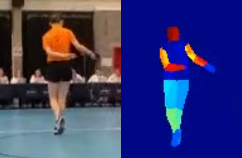
\includegraphics[width=0.3\linewidth]{../graphics/sr-denseposed}
    \caption[Image vs Densposed image]{Jumper in a routine wrapping the rope around her arm in a single rope routine. Image on the left is the original image, on the right is the simplified information after using detectron2 densepose \autocite{wu2019detectron2}}
    \label{fig:srwrap-bp}
\end{figure}

Densepose seems to be able to give the bounding boxes of the main poses detected. Perhaps just a convex hull and some padding will be enough for smart cropping and training a network from scratch is not needed.
However, a local tryout (without boxes) was rather slow, 1.2 fps on GPU within a Docker container.
As jumpers don't move that much most of the time, skipping some frames and smoothing out the prediction over the rest of the sequence or decreasing the amount of skipped frames when movement is detected can speed up the localization.

Even when Densepose isn't used, smoothing can still be applied to the guessed box as a video is basically a sequence of images.


\section{Video action segmentation}
\label{lit:video-action-segmentation}

When the athletes are cropped, videos need to be split \footnote{Not real/physical splits, but rather labels/annotations for where to split} in (sub)skills, because splitting new videos manually takes too much time and is impractical on competitions. A more specialized model like LTContext \autocite{Jiaming_2023} or a video vision model explored in section~\ref{subsec:bp-skill-recognition} could suffice.

Just like in localization, extracting poses, filtering foreground from background etc. could improve the segmentation.

The model for generating skill snapshots will
be useful for judging and subsequently labeling
data. Rather than replaying the video, judges can
just sequentially go through each trick one at a
time to assign, annotate or validate the predicted
skill.




\section{Skill recognition}
\label{lit:skill-recognition}

The final step would be to recognize the total skill in a freestyle video.
\textcite{Yin_2024} did a general HAR survey, mainly focused on team sports, in which they describe the evolution from normal CNN architectures, to recurrent neural networks for time sequences, remembering context, like the Long Short Term Memory model (LSTM), after which models were developed feeding the CNN output into LSTM or even implementing a convolutional filter in the memory cell \autocite{Shi_2015}.

\textcite{Wang_2019} investigated an improvement for current convolutional or recurrent models. They found that LSTM memory cells were too simple to contain higher-order complexities. As a result, they designed a memory in memory component, to replace the previous cell, which could predict actions on complexer data sets. This quickly formed the name Memory in Memory, MIM. Later, \textcite{Lin_2020} used a self-attention memory cell inside the convLSTM that can memorize global aspects in space and time. With about 35\% the number of parameters compared to Wang's MIM-model, SAM achieved a similar score as on the moving MNIST dataset, but faster. Although the focus of these papers was predicting future actions, the output can be transformed into a classification model, rather than a prediction model.

Another approach would be using transformers as a described  in \textcite{Yin_2024}. Options are the video vision transformer \autocite{Arnab2021} or adaptions like the ViT-TAD model by \textcite{Yang_2023}, Swin transformer \textcite{Liu_2021} or VideoMAE v2 by \textcite{Wang_2023}. Further research/try-outs will be required to ensure the transfer models can predict actions.

For reference, NextJump uses a CNN - MobileNetv4, \autocite{MobileNetv4_2024} and a transformer to analyze the full sequence and count. So using the convLSTM, SAM, MobileNet, or a transformer brings us to a better definition or example of what exactly we want to predict.

% TODO : SA_ConvLSTM?
% TODO : MViT

Even with a broad range of options, it isn't bad to think about potential hurdles. One of them are unknown of unusual skills. While a judge may refer to a head judge or think for itself, the AI model wouldn't be trained for that. The other hurdle could be that DD3 freestyles are a group activity, making it hard for models to recognize the required aspects. 

\section{Group activity}

As DD3 is a group activity, problems could arise while trying to detect skills. However, the hypothesis is that a DD3 freestyle always acts as one unit, thus not really requiring much special attention. One potential problem could be not know left from right, as there are two turners. Other problems might arise when adapting SR to SR2 where two individuals are not exactly one unit. Some further research can be done in models like stagNet \autocite{Qi_2020} to account for this idea. Another idea would be to apply the same method as YOLO, predicting multiple locations at the same time.




\section{Unknown/Unusual skills}
\label{lit:unknown-unusual-skills}

% TODO revise
Unknown skills or special cases pose another challenge. That's why the skill-matrix needs to defined in such a way, to accommodate for new combinations or skills. This is called zero-shot learning, \autocite{Pourpanah_2022}, where actions or combinations get recognized without any labels.

(Sort of marking unique skills as "I don't know" so that others new/unique ones will also be marked as "I don't know") Unusual skills on the other hand should be incorporated into the implementation.
A more concrete example would be turntables, which are mainly performed using a crab or push-up, but also seen with a frog or a split.
Turntables even have the potential to be combined with a swift. Omitting turntable frogs or splits in the train dataset can test this the ability to perform on unusual skills.




\section{Summary literature}
\label{lit:-summary-literature}

According to the state of the art, it appears feasible to analyze the performed skills in a given recording. In order to evaluate this, a proof of concept will be developed predicting jump rope skills. Sequentially, three steps are be required. The first step involves localizing the position of the athletes. This way, computational resources can be spared in the following steps, namely segmenting and recognizing. The segmentation consists of predicting split moments which should divide the video into likely skills. In the final step, the recognition step, each seperated skill can be analyzed by a vision model, predicting the most likely skill performed for the given section.

When all skills are predicted, corresponding levels and numeric scores can mapped onto each skillsection. These scores add up to difficulty score, usable to decide a victor on competitions.
%%=============================================================================
%% Methodologie
%%=============================================================================

\chapter{\IfLanguageName{dutch}{Methodologie}{Methodology}}%
\label{ch:methodologie}

%% TODO: In dit hoofstuk geef je een korte toelichting over hoe je te werk bent
%% gegaan. Verdeel je onderzoek in grote fasen, en licht in elke fase toe wat
%% de doelstelling was, welke deliverables daar uit gekomen zijn, en welke
%% onderzoeksmethoden je daarbij toegepast hebt. Verantwoord waarom je
%% op deze manier te werk gegaan bent.
%%
%% Voorbeelden van zulke fasen zijn: literatuurstudie, opstellen van een
%% requirements-analyse, opstellen long-list (bij vergelijkende studie),
%% selectie van geschikte tools (bij vergelijkende studie, "short-list"),
%% opzetten testopstelling/PoC, uitvoeren testen en verzamelen
%% van resultaten, analyse van resultaten, ...
%%
%% !!!!! LET OP !!!!!
%%
%% Het is uitdrukkelijk NIET de bedoeling dat je het grootste deel van de corpus
%% van je bachelorproef in dit hoofstuk verwerkt! Dit hoofdstuk is eerder een
%% kort overzicht van je plan van aanpak.
%%
%% Maak voor elke fase (behalve het literatuuronderzoek) een NIEUW HOOFDSTUK aan
%% en geef het een gepaste titel.

This section contains a brief description of the road map to build the proof of concept (PoC), which combines the general key insights from the literature. Within the methodology a brief description is provided about each experiment, without specifying actual results or code implementations. These can be found in \ref{ch:results}

The proposed model can be seen as a three-way modular setup, jumper localization, action segmentation and skill recognition.
Each step can be improved individually in order to acquire the best possible result and is implemented independently.
The first step focuses on localizing the athletes in the field in order to crop them out and spare computational resources. Next up is segmenting each skill performed in a given routine. The final part involves recognizing each isolated skill.

All experiments are performed using an Acer Nitro ANV15-51, running Ubuntu 24.04.2 LTS, using a 13th Gen Intel® Core™ i5-13420H × 12, with 16GB RAM and a NVIDIA GeForce RTX™ 4050 Laptop GPU 5898MiB.

% TODO : chart overview of model.

\section{Genral information}

Before jumping into each different step, some general information is provided. Each of the 458 DD3 freestyles collected, 2231 total videos, has a record in the database. Two selections have been made to decide the videos in the validation set. The first selection is filtering all videos of this season (67 videos). The second selection uses the id of the video. In the beginning of the project, taking the 10th modulo of the id being 5 resulted in the most validation videos. Currently this corresponds to 42 validation videos. The other 90\% are used as training videos (349).
Each recording lasts for about 60 to 75 seconds, depending on the competition level and has around 40 to 60 performed skills. These do not include normal jumps. In order to annotate the videos, a custom Vue3 web application is created. In order to render the videos in the browsers, conversions from blu-ray (m2ts) or AVI to mp4 were required. Most videos have a framerate of 25, 30 or 50 frames per second (fps), while some may be 15, 28 or 60.
The quality of videos differ and range from anywhere between 8 and 550MB. It may not indicate much, but just to keep in mind. Even on the more qualitative videos, the rope disappears when making quick rotations. This is often better on higher fps videos.

\section{Jumper localization}
\label{methodology:jumper-localization}

Jumper localization is needed in order crop a zoomed-in video of the skippers performing their routine. Image \ref{fig:sr4-field} perfectly illustrates a competition setting, where the majority of the video is lost on surroundings, judges and spectators. The field is typically 12 by 12 meters for the athletes to use.

\begin{figure}
    \centering
    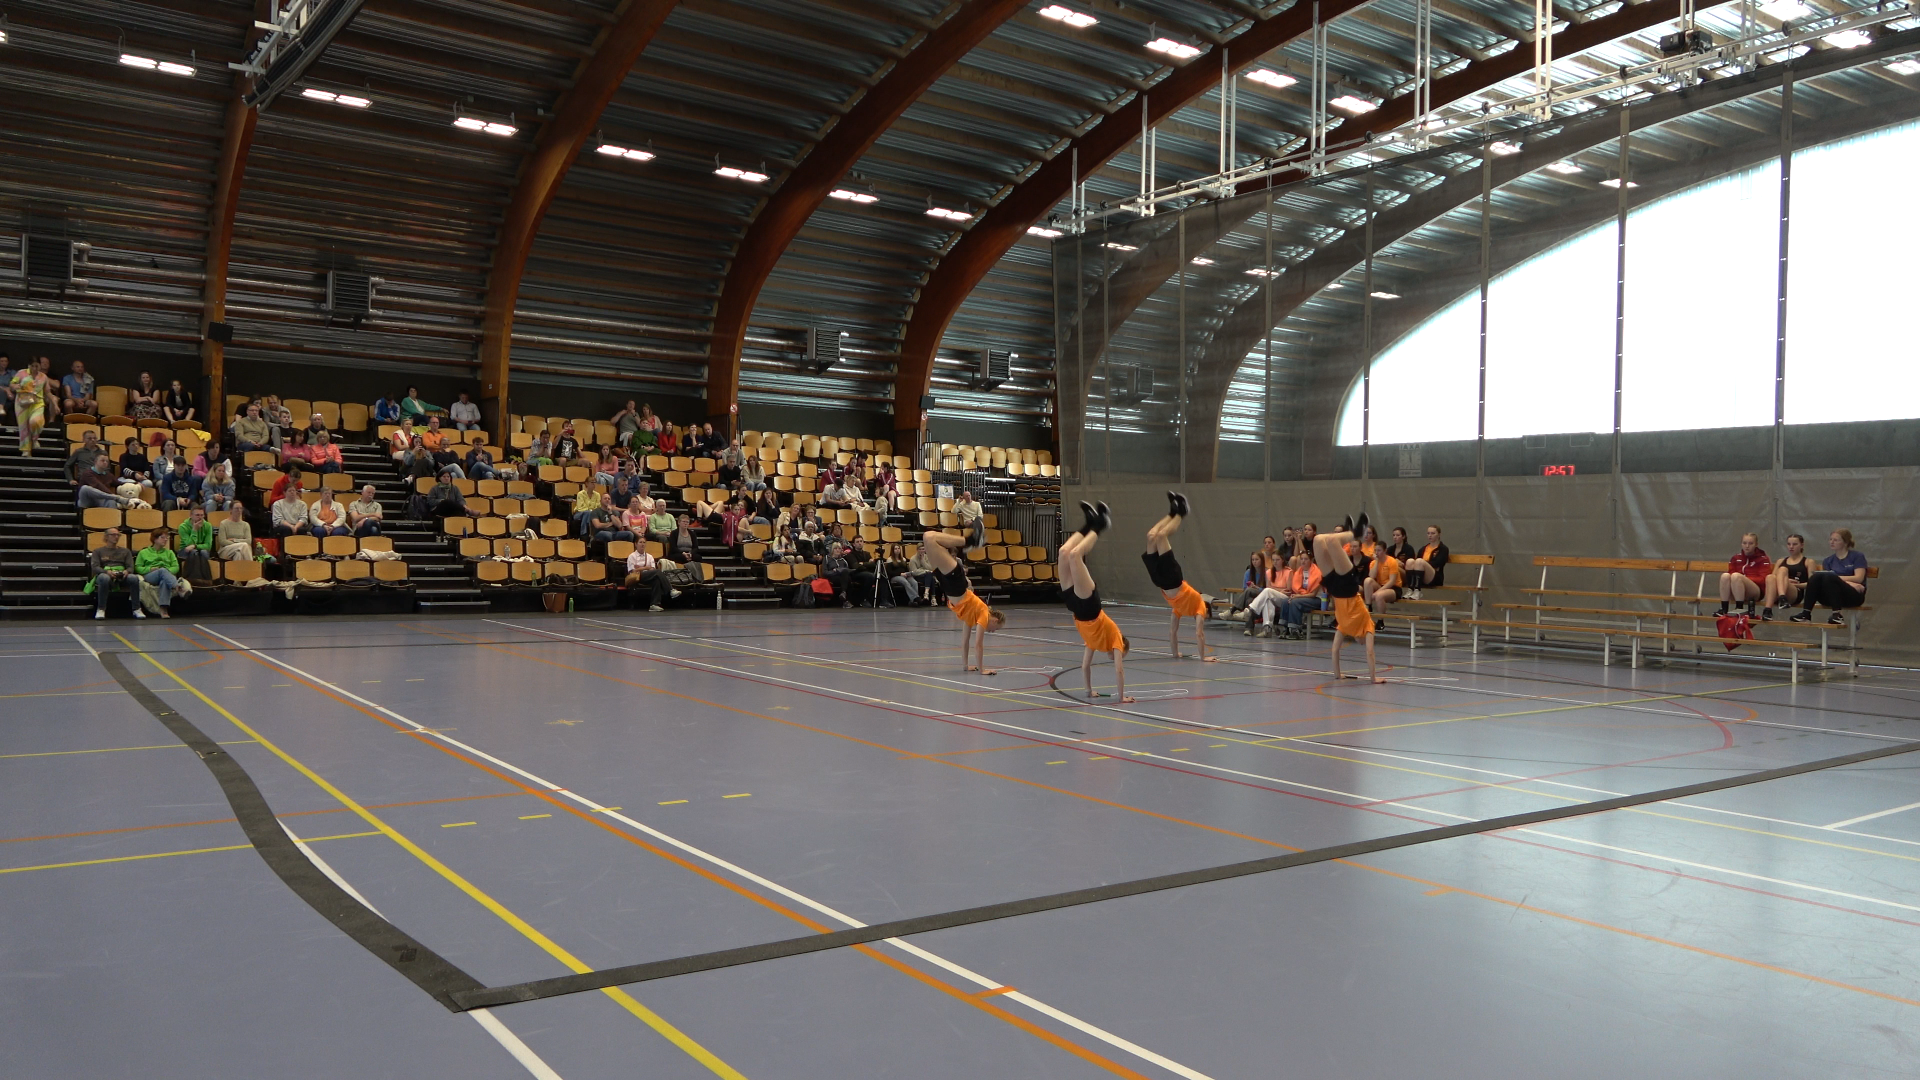
\includegraphics[width=0.95\linewidth]{sr4-field}
    \caption[Example jump rope competition setting]{Example of a competition setting in which four athletes are performing a SR4 freestyle.}
    \label{fig:sr4-field}
\end{figure}

Experiments on localizing implement two major ways of labeling athlete locations, full team boxes and individual boxes.
For this project the relative center point along the x-axis, y-axis, width and height of the box are stored. So regardless of the scale of the image, whether the image has size 1920 x 1080 pixels or 1080 x 720 pixels, the position of the box remains the same.
This way, by scaling all images to the same size, frames of dimension (width, height, channels) can fed into the model \ref{code:keras-random-conv}, giving 4 values in return. An example of a box would be [0.6, 0.5, 0.4, 0.4], all values range between 0 and 1.
Team labels require one box for a single image, contrary to multiple boxes for individual athletes. 
After training and predicting box coordinates, the Jaccard similarity coefficient otherwise known as the Intersection over Union accuracy (IoU) can be performed evaluating the performance of the model. This allows for comparison of models or training rounds.

Full team predictions were experimented on MobileNetV3 \autocite{Howard2019} and GoogleNet \autocite{Szegedy2014}. Labeling some frames of almost any DD3 routine, variety in the leftover data was limited. This marked the transition towards individual labels.

% TODO Vision Transformer?
Ultralytics, \autocite{Khanam2024}, provides an easy way to implement their YOLO models. For this research, YOLOv11 is used to predict individual boxes, providing satisfying results \ref{results:yolo}. 
Using the predicted locations of the skippers, each frame of video can be cropped around the athletes. Results weren't perfect, sometimes visual disturbing, because of sudden zoom outs, blurry athletes or predictions of spectators. This required smoothing techniques to improve full video crops \ref{results:crop-stability}.

Manually reviewing full cropped videos is time consuming, requiring automated tests in order to check full video crops. The implementation of these automated tests used the full team boxes comparing the minimum IoU overlaps for each video, as these moments mattered most. By manually checking videos, problematic moments were additionally labeled as full team boxes. However, the further development and full video crop results were unfinished and put on hold due to time constraints. 

\section{Action segmentation}
\label{methodology:action-segmentation}

The main purpose of the action segmentation is to enable predictions on full routines in order to actually use the whole model. Using the cropped images, and the assigned start and end frame of a skill, the model can predict whether a given frame is an interesting split point or not.

For jump rope, this mostly means moments when an athlete leaves or lands on the floor. However there are special cases such as cartwheels. Only moments when either hands or feet land over a rope, are annotated as the end of a skill. 
To annotate which moments are interesting split points, the start and end frame of a skill receive value 1, while other frames remain 0.
As the start and end frame of a skill are rather subjective, frames around a split point also range somewhere between 0 and 1. These values are calculated using the function \ref{code:calculate-splitpoint-values} which is called on in the data generator demonstrated in code \ref{code:call-splitpoint-calculation}.
Each frame than has a value from zero to one. An example of consecutive splitpointvalues could be:

\([0, 0, 0.1, 0.31, 0.55, 0.86, 1, 0.86, 0.55, 0.31, 0.1, 0]\)

Having a splitpoint value for each frame of the video, the video can be partioned into consecutive sections of T timesteps. Because the Multiscale Vision Transformer is pre-trained on videosections of 16 frames, the same amount of timesteps are taken to finetune the model for segmentation. This makes the model transform the input of size (batch size, channels, timesteps, height, width) into an output of size (batch size, timesteps).

Available experiments include code implementations of the Video Vision Transformer as introduced in \textcite{Arnab2021} (ViViT - \ref{code:get_model_ViViT}) and the Self-Attention ConvLSTM from \textcite{Lin_2020}. Both models showed the same results, averaging out predictions slightly above 0 for all frames, stagnating on MSE losses, not actually grasping what happens in given sections of frames it receives.

The final experiment on action segmentation uses \href{https://pytorch.org/vision/main/models/video_mvit.html}{PyTorch's Video MViT}, which is an implementation based on the Multiscale Vision Transformer created by \textcite{Fan2021} which can be finetuned using the pre-trained weights on the kinetics dataset \autocite{Kay2017}. This experiment will be elaborated in section \ref{results:action-segmentation-mvit}.


\section{Skill recognition}
\label{methodology:skill-recognition}

The last part involves recognizing each performed skill, which is, as introduced in the literature, a combination of different aspects. What are the turners doing, using one or both arms, an additional body rotation, etc.
For this part, a video vision model is definitely required to fill in the temporal information, e.g. amount of rotations.

One minor issue, is about skills differing in duration. One might take half a second, the other might be 800 milliseconds.
This can be solved by ensuring they have the same length of T = 16 timesteps, skipping or duplicating frames. This resulted in equal sized inputs with dimensions (channels, timesteps, height, width) or (C, T, H, W) for short.

Next up was transforming all aspects of skills into machine understandable output labels. This was the reason why the skill matrix has been created \ref{lit:skill-matrix}. The matrix resulted in a skill configuration \ref{code:confighelper} for skill labels, specifying 13 different outputs; Type, Rotations, Turner1, Turner2, Skill, Hands, Feet, Turntable, BodyRotations, Backwards, Sloppy, Hard2see and Fault. Each aspect being a category, numeric value or a boolean.

Along the way, additional aspects to a skill label can be added in order to incorporate for every level and skill variation.
Furthermore, once-in-a-lifetime skills can be marked as unknown in order for the model to be robust in predicting new skills. After analyzing the given skillsection, a level can be assigned, based on the predicted aspects.
Multiple different models can be tested in order to find the best one.

The first experiments implement the Video Vision Transformer and the Self-Attention ConvLSTM, which averaged out the most occuring aspects; normal jumps, no mistakes, 1 rotation...
These models were trained on upsampeled data, increasing occurances of more unique skill combinations.

Following unsuccesful trials trained from scratch, accelerated the implemenation of the Multiscale Vision Transformer for recognizing skills. At the same time, in order to test things out, skills where limited to to a balanced 5 class datataset; jumps, return from powers, pushups, frogs and other skills, hoping for better results.
The results where excellent, even starting to recognize aspects of turners, quickly re-enabling predictions on all skills \ref{results:mvit}.

Further experiments added other models, namely video ResNet models or Swin Transformers \ref{results:skill-recognition-resnet-swin-saconv3d} or adjusted the returned losses, based on skill aspect occurance in the dataset during training and validation \ref{results:skill-recognition-weighted-losses}. 

\section{Judge score comparison}
\label{methodology:judge-score-comparison}

Finally, when skills are predictable, a comparison between the jury assigned scores, the models prediction and the effective score can be made in order to check whether model predictions could be used or more research/training is needed. This is an important check, verifying usability on competitions \ref{results:skill-recognition-act-as-a-judge}.



% Voeg hier je eigen hoofdstukken toe die de ``corpus'' van je bachelorproef
% vormen. De structuur en titels hangen af van je eigen onderzoek. Je kan bv.
% elke fase in je onderzoek in een apart hoofdstuk bespreken.

%\input{...}
%\input{...}
%...
%%=============================================================================
%% Results
%%=============================================================================

\chapter{\IfLanguageName{dutch}{Resultaten}{Results}}%
\label{ch:results}

The result section focuses on elaborating conducted experiments and acquired results, divided into the three main phases, localization, segmentation and recognition. In order to label, annotate videos and gain insights in the results a Vue3 web-app is created on a python flask API which reads and stores labels and video annotations from a MySQL database. Furthermore, the experiments are all performed using an Acer Nitro ANV15-51, running Ubuntu 24.04.2 LTS, using a 13th Gen Intel® Core™ i5-13420H × 12, with 16GB RAM and a NVIDIA GeForce RTX™ 4050 Laptop GPU (6GB).

\section{Jumper localization}

% TODO: add, this is relevant
% TODO: convex hull the 3 jumpers and train on yolo model.
As DD3 routines are the focus of this research, the idea to predict the location of the whole team instead of individuals was made. As there aren't any public jump rope labels, the idea was that this would increase labeling speed. Predicting full teams didn't work out which allowed for a transition to labeling and predicting individuals athletes. Below you find more information about the following experiments.

1. Labeling boxes 4 all jumpers -> training models (from scratch). -> low accuracy, naive bias.
1.1 random conv
1.2 googlenet, mobilenet...

2.0 Mask-RCNN
2.1 Labeling individual jumpers \& pre-trained model yolo -> OK

\subsection{Box coordinates}

Before discussing the different results, let's discuss how the location of skippers are marked.
... Image, full team vs individual coordinates.
XYXY vs CenterX CenterY W H.
How to measure accuracy -> IoU.

\subsection{Random convolutional network}
To get a first idea whether it would start learning, so a transition can be made towards more advanced architectures.

\subsection{Dedicated architectures}
GoogleNet, MobileNet... (on individual labels)

\subsection{Mask-RCNN}
Failed experiment, C error, no results.

\subsection{Jumper localization using YOLO}

Ultralytics \autocite{Khanam2024} provides an easy to use implementation for predicting people and objects in images which can be fine-tuned for specific use cases. Fine-tuning was needed as spectators, also humans, were also being predicted as athletes. Using these predictions, a crop around the three jumpers can be created using the predicted jumper boxes from the fine-tuned YOLO model, after using the pre-trained weights on the COCO dataset \autocite{Lin2014}. In order to improve the crops some steps were required. They may not be perfect, but it works for now.

\subsection{Eliminate spectators - IoU comparison}

In order to make te best possible crop there are probably thousands of methods. The current implementation involves taking the minium and maximum x- \& y-coordinates to draw the box containing all skippers.
At this moment, it is expected that the YOLO model has been fine-tuned to distinguish athlete and spectator.

Even though the model is fine-tuned on almost two-thousand images, occasionally coaches or spectators were still predicted as jumpers, requiring a solution.
When a spectator or more than one is predicted, this means that total crop of all 'athletes' could be bigger than the actual location of all jumpers. A comparison in overlap between previous predictions (N seconds) and the current prediction enables the possibility to keep the crop position of the previous frame for the current frame. Comparing overlap is called Intersection over Union or IoU for short.

(Clarifying images will follow in a next version)

A possible improvement could be matching previous boxes with the new predictions, eliminating the spectator. Which begs the question, what if the jumpers are entering the field? There are no earlier predicted boxes to match.

\subsection{Eliminate shakiness}

A video is a sequence of frames changing the position of the skipper a little bit each frame. Even if actions are fluidly executed, the actual predictions of the jumpers location can shift a few pixels to the left or right between consecutive boxes. This means that raw crops are shaking around the jumper, disturbing the natural feel.

Smoothing values (S), two parameters, where added to eliminate the shaking of consecutive crops. One of the parameters is used for smoothly shrinking the frame (0.94), the other for expanding the frame (0.85).
This means that the crop of a new frame is S times the crop value of the previous frame added with 1 - S times the new prediction, elimination shakiness. The second parameter was added in order to fix jumpers running out the crop while executing a larger actions covering a lot of position on the floor.

It was playing around with these parameters (smooth values \& N) to get a working setup which works in most cases, sporadically changing one if the crop of a video was not sufficient, e.g. running out of the cropped view.


% \begin{listing}
%    \begin{minted}{python}
%        import pandas as pd
%        import seaborn as sns

%        penguins = sns.load_dataset('penguins')
%        sns.relplot(data=penguins, x="flipper_length_mm", y="bill_length_mm", hue="species")
%    \end{minted}
%    \caption[Voorbeeld codefragment]{Voorbeeld van het invoegen van een codefragment.}
%\end{listing}


\section{Action segmentation}

\section{Skill recognition}

The first trials from scratch, a video vision transformer, which is adapted from the transformer created during classes. Adding the convolution layer in front and the time dimension created the ViViT transformer as proposed in (source).
Idea's add extra convolution layers \& use pre-trained model.

Elaborate 16 frame time aspect.

\subsection{Video Vision Transformer}

For training the video vision transformer, the data is upsampeled

\subsection{Multiscale Video Vision Transformer - MViT}
\href{https://pytorch.org/vision/main/models/video_mvit.html}{Pytorch MViT}

Pytorch implementation of source.

For the first training round a double upgrade has been performed. The first adaption is downsampling the skills in 5 main classes to predict.  \& pre-trained model.

\begin{table}[h!]
    \centering
    \begin{tabular}{|r|r|l|r|r|}
        \hline
        \textbf{Train \%} & \textbf{Train Count} & \textbf{Skill} & \textbf{Val Count} & \textbf{Val \%} \\
        \hline
        50.6687 & 2273 & jump & 379 & 56.6517 \\
        14.0660 & 631 & pushup & 77 & 11.5097 \\
        13.0629 & 586 & return from power & 84 & 12.5561 \\
        9.8529 & 442 & frog & 59 & 8.8191 \\
        3.2100 & 144 & crab & 9 & 1.3453 \\
        2.0062 & 90 & split & 12 & 1.7937 \\
        1.1146 & 50 & flip & 5 & 0.7474 \\
        0.9140 & 41 & rondat & 5 & 0.7474 \\
        0.8917 & 40 & rad & 3 & 0.4484 \\
        0.8025 & 36 & suicide & 8 & 1.1958 \\
        0.7356 & 33 & handspring & 5 & 0.7474 \\
        0.6910 & 31 & rol2kip & 7 & 1.0463 \\
        0.4458 & 20 & kip & 6 & 0.8969 \\
        0.3567 & 16 & speed & NULL & NULL \\
        0.3121 & 14 & kopkip & 1 & 0.1495 \\
        0.2675 & 12 & roll & 3 & 0.4484 \\
        0.1783 & 8 & stut & 2 & 0.2990 \\
        0.1337 & 6 & swift & NULL & NULL \\
        0.1337 & 6 & UNKOWN & 1 & 0.1495 \\
        0.0669 & 3 & leapfrog & NULL & NULL \\
        0.0446 & 2 & footwork-kick & NULL & NULL \\
        0.0223 & 1 & mountainclimber & NULL & NULL \\
        0.0223 & 1 & footwork-open & 1 & 0.1495 \\
        \hline
    \end{tabular}
    \caption{Skill distribution with training and validation counts and percentages. Null values indicate missing validation data.}
    \label{tab:skill_distribution_full_with_nulls}
\end{table}


\begin{table}[h!]
    \centering
    \begin{tabular}{|l|r|r|r|r|}
        \hline
        \textbf{Skill} & \textbf{Train Count} & \textbf{Train \%} & \textbf{Val Count} & \textbf{Val \%} \\
        \hline
        jump & 2273 & 50.6687 & 379 & 56.6517 \\
        pushup & 631 & 14.0660 & 77 & 11.5097 \\
        return from power & 586 & 13.0629 & 84 & 12.5561 \\
        frog & 442 & 9.8529 & 59 & 8.8191 \\
        other & 526 & 11.7253 & 68 & 10.1645 \\
        \hline
    \end{tabular}
    \caption{Train and validation skill distribution with low-frequency skills grouped as "other"}
    \label{tab:skill_distribution_grouped_final}
\end{table}


\section{Model verification}

%%=============================================================================
%% Conclusie
%%=============================================================================

\chapter{Discussion}%
\label{ch:discussion}

% TODO: Trek een duidelijke conclusie, in de vorm van een antwoord op de
% onderzoeksvra(a)g(en). Wat was jouw bijdrage aan het onderzoeksdomein en
% hoe biedt dit meerwaarde aan het vakgebied/doelgroep?
% Reflecteer kritisch over het resultaat. In Engelse teksten wordt deze sectie
% ``Discussion'' genoemd. Had je deze uitkomst verwacht? Zijn er zaken die nog
% niet duidelijk zijn?
% Heeft het onderzoek geleid tot nieuwe vragen die uitnodigen tot verder
%onderzoek?

The goal of this research was to increase in the objectivity and accuracy of scores assigned by judges on jump rope freestyles during competitions using recent advancements in machine learning technology.
In order to achieve this, two sets of questions needed answers.
The first set being questions about jump rope, which will be answered in \ref{ch:discussion-jump-rope-answers}. The second set contains questions about the machine learning part, which follows in \ref{ch:machine-learning-answers}. Some of them required an answer before starting the development of the proof of concept, while others depended on the PoC.

\section{Jump rope answers}
\label{ch:discussion-jump-rope-answers}

Today, the challenge for jump rope judges \ref{intro-bp:question-challenges-for-judges} is the ability to keep up with the skills performered, while calculating the skill level, in order to accurately score the difficulty of a routine. In order to reduce errors, judging methods change, such as adapting the rules \ref{lit:adapting-the-rules} or reviewing the routine post-performence at slower speeds \ref{lit:review-at-slower-speed}.

Skills were then broken down \ref{lit:jump-rope-skills-introduction} to better understand how difficulty is scored \ref{intro-bp:question-difficulty-scored}. These were further specified and organized into a skill matrix \ref{lit:skill-matrix} in order to specify which exact actions needed to be recognized \ref{intro-bp:question-what-are-the-skills-to-be-recognized}.
Having skills specified, leads to the machine learning part, transforming this matrix into computer output and exploring machine learning possibilities. % possibilities / results?


\section{Machine learning answers}
\label{ch:machine-learning-answers}

% TODO add sensoric data if time?
Computer vision \ref{lit:computer-vision}, a subset of machine learning, is the ability of computers to understand visual data.
Exploring this topic; models, other sports, the jury support system of Fujitsu (\ref{intro-bp:question-earlier-research-guidance}, \ref{lit:computer-vision-sports}), the availability of video recordings (\ref{intro-bp:question-data}, \ref{tbl:data-comparison-sr-dd}), along with aquiring information about and NextJumps' speedcounter \ref{lit:nextjump-speedcounter} allowed for the choice to learn out of video material \ref{intro-bp:question-which-modern-technologies}.

Using videodata and recognizing actions required to think about quite some properties. Recordings are typically full routines of about 60 to 75 seconds. These freestyles contain 40 to 60 skills, around 100 if you include normal jumps. Some recordings are zoomed-in, others are stationary capturing the whole field. The videotype may be mp4, blu-ray (m2ts) or AVI. Even the framerate could differ (25, 30, 50).
Considering these aspects, a general approach for recognizing skills in a video is created while exploring human action recogniton \ref{lit:human-action-recognition}. This resulted in three steps; jumper localization \ref{lit:jumper-localization}, action segmentation \ref{lit:video-action-segmentation} and skill recognition \ref{lit:skill-recognition}, each of them requiring future work \ref{discussion:future-work}.

% TODO : add refs to methodology or results?

\subsection{Localization}

Localization serves as a way to zoom in and focussing on the actions, sparing computational resources, rather than providing frames to a model where the actions and athletes only take up a limitted amount of space in the video \ref{fig:sr4-field}.

on the  Tests on results for localizing \ref{results:jumper-localization} are limited in order to have spent sufficient time for segmenting and recognizing skills. Even then, time was limited. Predicting the location of jumpers has been tested using full boxes as a first stage. Models in this stage included MobileNet and GoogleNet, but results were lacking. The switch to annotate individuals instead of full teams and using a pre-trained YOLO model quickly reached better results.
Even though the mAP50 reached 0.943 accuracy, intial full videocrops weren't stable, requiring smoothing techniques and more labels in order to reduce spectator predictions and visually disturbing shocks (table \ref{tbl:crop-results}). Utilizing a basic smoothing technique \ref{results:crop-stability} allowed for sufficient videocrops, which can be used for skill recognition \& segmentation.

\subsection{Future work on localization}

Localization can be improved in multiple areas. This could involve training on full team labels using YOLO, applying other smoothing techniques or implenting other models. Other factors could be changing the competition setting to limit the amount of spectators, keeping the camera perspective consistent or provide more different perspectives. Another way is annotating the predicted spectators or judges, indicated by pre-trained models, which can be filtered out when cropping.

\subsection{Segmentation}

The part about action segmentation definitely needs more research and experiments. The easiest implementation was utilizing vision models used for recognizing actions to annotate interesting split points having a value of 1, a split moment, or 0, executing a skill or doing nothing. Using the Multiscale Vision Transformer, developed by \autocite{Fan2021}, which acquired great results recognition \ref{results:skill-recognition}, quickly showed overlap between predicted split points and labeled split points \ref{fig:segmentation-plot}.
The MViT applied for segmentation transforms the annotated skill labels \ref{methodology:skill-recognition} into split labels \ref{methodology:action-segmentation}. A little summary of the labels follows. Skills labels have a start and end frame, which allows to indicate split values at these frame numbers to be around one. An example would be:

\(
[0, 0, 0.1, 0.31, 0.55, 0.86, 1, 0.86, 0.55, 0.31, 0.1, 0, 0, 0 \dots]
\)

Videos were then split into partitions of T = 16 timesteps, learning some context of previous and following frames, in order to predict the corresponding T split output values as wel. The highest peaks were then considered split points \ref{fig:segmentation-plot}.
Being able to predict splitpoints allows to perform skill recognition on completely unseen videos, isolating each action.

\subsection{Future work on action segmentation}

Due to time constraints and priorities, only the MSE has been used to decide the most optimal split moments on the MViT model. There are still future actions which could improve action segmentation. Ideas, not limited to the list below, include:

\begin{itemize}
    \item Implement other metrics for segmentation next to MSE
    \item Wider or more narrow split point values.
        \begin{itemize}
            \item IoU section overlap
            \item Average distance to closest split point
            \item Count of predicted splitpoints vs actual splitpoints
        \end{itemize}
    \item Implement a second dimension, is jumping parameter to filter out mistake recoveries or non jumping moments.
    \item Predict every other frame, instead of all frames.
    \item Implementing a action segmentation specific models.
    \item More labels
\end{itemize}

\subsection{Recognition}

Being able to zoom in on athletes and having a model which can segmenting actions, actual skills can be predicted on full videos.
But even before the ability to isolate skills, labeling and training experiments on skill recognition are possible. One minor issue, solved in the methodology of skill recognition \ref{methodology:skill-recognition} was the fact that performed actions have a different length \ref{fig:skilllengths-counts}. This is solved by ensuring they have the same length of T = 16 timesteps, skipping or duplicating frames \ref{methodology:skill-recognition}. This resulted in equal inputs with a dimension of (channels, timesteps, height, width), (C, T, H, W) for short.

Next up was transforming all aspects of skills into machine understandable output labels. This was the reason why the skill matrix has been created \ref{lit:skill-matrix}. The matrix resulted in a skill configuration \ref{code:confighelper} for skill labels, specifying 13 different outputs; Type, Rotations, Turner1, Turner2, Skill, Hands, Feet, Turntable, BodyRotations, Backwards, Sloppy, Hard2see and Fault. Each aspect being a category, numeric value or a boolean.

The final adaptation using weighted losses, which returned a different loss depending on the occurrence of skill aspects pushed the MViT model into grasping the meaning behind the fault, sloppy and hard2see aspects. It raised the f1 average macro accuracy from 45.61\% to 51.53\%, giving in on f1 macro skill accuracy. It fell from 34.93\% to 27.75\%, which is low compared to the skill recognition accuracies on MViT extra dense 31.46\%, SwinT t 32.06\%, and SwinT s 36.73\%. However, it still reached highest on the normal accuracy measure 93.83\%, compared to 93.73\%, 91.99\%, or 93.3\%.

It is unknown how much data is expected to increase the accuracy \ref{intro-bp:question-expected-data-to-increase-accuracy}, but one major improvement is adding sufficient examples of each skill or turner, in order to provide enough feedback to model to learn more about these less represented skill aspects.

\subsection{Future work on skill recognition}

Aside from additional labels, some possibilities to increase accuracy are fine-tuning the weighted losses or experimenting using different models. Another experiment could be predicting the actions of individual athletes, instead of regarding the video section as a single unit. This can be especially usefull when predicting single rope team freestyles, in which the jumpers act as a unit, but also act as an individual, contrary to double dutch freestyles. Currently the data has been downsampled, filtering mostly normal jumps. This downsampling can be adjusted, as it there could be turner skills when there is a normal jump, limiting the training of these turners. Further data augmentation, besides mirroring the visual, such as color shifts, random crops or camera motion can also increase the accuracy of the models. A more difficult research topic, could be to create a full 3D pose of the athletes, which might require multiple cameras. 

\subsection{Judge score}

In the final run, MViT reached the best judge score results, with a difference of -21.68\% compared to the scores allocated by judges.
Time constraints didn't allow for a comparison of judge scores and model predictions with the ground truth. Thus the desired outcome to have a score difference around 5 to 10\% couldn't be measured. Even the -21.68\% is way to far off in order to use at competitions.

\section{Other future work}
\label{discussion:future-work}

When ground truths are available for the routines, an actual comparison between judge scores and models can be made to decide the better judge. Meanwhile, skill matrices for other events can be created, labeled on videos and trained, allowing for a broader range of models, model outputs and possibilities.

To conclude, this research showed the possibilities of the proposed three step architecture for recognizing skills in a full routine on a limited dataset. While results aren't perfect, great effort has been put in the proof of concept, enabling future research. The main priority should now be recording and annotating more videos, with different camera perspectives, including more skill of each skill variation in both the training and validation dataset.


%---------- Bijlagen -----------------------------------------------------------

\appendix

\chapter{Research proposal}

The subject of this applied thesis is based on the earlier approved research proposal. This submission is added as attachment.

%% TODO:
\section*{Proposal abstract}

    Judging jump rope freestyle routines at the highest competitive level has become increasingly challenging due to the evolution of jump rope. Both the number of skills that are included in a routine as well as the speed with which these are executed keep increasing. This is particularly evident in so-called Double Dutch Freestyle routines, which is why assigning scores to these freestyles is done by a combination of live and delayed evaluation. The creativity of a routine (including its variation and musicality) is scored in real time but the assignment of the appropriate difficulty level is done based on a recording of the routine replayed at half speed right after it is performed. Even though this helps reduce errors in difficulty scoring, a certain variability in the assigned scores persists/can still be seen. With the increased accessibility of artificial intelligence, particularly neural networks, the question arises whether an AI judge or assistant can be developed to obtain a more accurate (objective) difficulty scoring.

    This research explores the possibility and development of such an AI assistant, as well as the techniques and challenges required to obtain the desired level of objectivity.
    The current idea is divided into three sections. The first section will be localizing the jumpers in the field as most obtained recordings are not fully zoomed in or recorded using a static camera. As recorded jumpers sometimes take up less than a fifth of the recording, they can be cropped out sparing computational resources for the parts to come. The second part involves isolating skills from a routine into individual skills or subskills. This enables the assistant to not only label a single skill, but also dozens of skills performed sequentially without interference. Lastly, each segment can be assigned to its corresponding skill. For Double Dutch Freestyles this means the combined action of jumpers and turners resulting in a large possibility of unique combinations. By further marking presentational skills or difficult to see skills as unknown (e.g. when one athlete stands between others and the camera) it is expected that the AI judge will indicate unknown or unclear skills by itself. This way the the assistant can be put into practice when reaching similar or more accurate results than the live jury panel. The assistant's results allow for verification of scores during and after the competition, increasing transparency and accuracy even further. Using the current obtained competition videos displaying the most common skills a few hundred times, it is expected that the AI judge will start to distinguish between skills like a cartwheel, split or salto.
    In case it works, it is not only useful for jump rope freestyles but also applicable in other judge-related competitions such as gymnastic routines, figure skating, or synchronized swimming.

% Kopieer en plak hier de samenvatting (abstract) van je onderzoeksvoorstel.

% Verwijzing naar het bestand met de inhoud van het onderzoeksvoorstel
%---------- Inleiding ---------------------------------------------------------

\section{Introduction}
\label{proposal-sec:proposal-introduction}

Jump rope is an evolving sport.
Year after year, an increasing amount of high-level competitors are pushing the limits of jump rope.
% TODO : source?
This results in new skills, new combinations, better physiques, better rope material, and faster movements. For the judges to keep up with the jumpers and to correctly assess scores to a routine, Double Dutch freestyles\footnote{Two turners, with one or more jumpers} are reviewed at half speed in International competitions or even at nationals in Belgium.

Head judges around the world question the best way to judge athletes correctly so as to give an accurate and objective ranking in national or international competitions.
Many solutions have been provided: another judging rule set\footnote{The current rule set is enforced and maintained by \href{https://www.gymfed.be/}{Gymfed}, closely related to the international judging-rules from the \href{https://ijru.sport/}{International Jump Rope Union}}, splitting judge responsibility, replaying the routine at half speed \dots

However, with the increasing popularity of image recognition, more powerful computers, applications that recognize objects in images \autocite{Singh_Gill_2022}, implementations detecting simple human actions \autocite{LUQMAN_2022}, examples of action recognition in other sports \autocite{Yin_2024} and the successful test of \href{https://nextjump.app/}{NextJump}'s AI speed-counter, head jurors wondered about the possibility of using modern technologies like artificial intelligence to improve the judging results of jump rope freestyles.

This results some in the main research question of this paper: \textbf{``How can artificial intelligence be incorporated into jump rope freestyles to increase the objectiveness and accuracy of judging?''}.

\subsection{Problem domain}
\label{proposal-subsec:proposal-intro-problem-domain}

Jump rope, like gymnastics or athletics, exists in many disciplines like Speed, Single Rope freestyle (single/pair/team), Chinese Wheel (CW) or Double Dutch (single/pair).
To accurately judge routines, each discipline has its own rules. Although interlapped, differences exist. Each athlete or team then performs a choreography of 60 to 75 seconds showcasing their favorite skills and uniqueness.

\subsubsection{What are the challenges for judges today?}
\label{proposal-subsubsec:proposal-intro-question-challenges-for-judges}

On competitions, judges watch the routine live to annotate the difficulty or creativity. Each judge then pays attention to his assigned part, e.g. movement, musicality or difficulty, all of those elements contributing to the total score of the freestyle. The main problem now is for judges to keep up with double dutch routines. Single rope freestyles are still manageable. To increase the accuracy, difficulty-certified judges \footnote{Those judges judging the difficulty of double dutch routines.} are already allowed to review freestyles at half speed in order to score them accurately.

\subsubsection{How is difficulty scored?}
\label{proposal-subsubsec:proposal-intro-question-difficulty-scored}

Performed skills each have a level, which will be written down when seen by the judge. Each level also has a numeric score that contributes to the total difficulty of the routine. Judges see and calculate/memorize the level of each skill, write it down, count the number of levels jumped and calculate the diff score.

\subsubsection{What are the skills and transitions that need to be recognized?}
\label{proposal-subsubsec:proposal-intro-question-what-are-the-skill}

% TODO : provide examples of skills
For double dutch, there are two turners and at least one jumper. All three of them act as a unit and execute skills or turner combinations. Jumpers can do a handstand, push-up or a cartwheel, while turners can turn with their arms crossed, on the back or rotating two ropes underneath the jumper at once. Furthermore, combining skills of a jumper while doing a special rotation contributes to more difficulty and more points. Even different transitions like a turntable, which is a push-up to a push-up while your body position changes a quarter is a different transition.


% TODO : omit or shift
%\subsubsection{What can be done to increase the accuracy of judging?}
%\label{proposal-subsubsec:intro-question-how-to-increase-accuracy}

% The preferred solution in this proposal is an AI-model recognizing (sub)skills and transitions in a double dutch single freestyle (DD3) as assigning correct levels at world championships or even nationals in Belgium is perceived to be hard and the current main issue.


\subsection{Solution domain}
\label{proposal-subsec:proposal-intro-solution-domain}

Until now, only the scope has been narrowed down. The focus will be put on double dutch freestyles. Getting to know the topic is great, but this doesn't get us further into the solution. Let's jump into it.

% TODO : update order
\subsubsection{Which modern technologies can be used to increase score accuracy of jump rope freestyles}
\label{proposal-subsubsec:proposal-intro-question-integration}

As reviewing routines at half speed still has his limits, using machine learning (an AI-model) could reduce time spent on judging routines. The idea would be a machine learning model recognizing (sub)skills and transitions in a double dutch single freestyle. (DD3)

\subsubsection{Which data is available for the machine learning model to use?}
\label{proposal-subsubsec:proposal-intro-question-data}

To recognize hundreds of skills, variations and transitions, lots of data is needed. Both individual and team freestyles are mostly recorded by clubs themselves or event organizers, some which are available on social media. The task is to explore and gather as much as possible.

\subsubsection{When are predictions acceptable to potentially use on competitions?}
\label{proposal-subsubsec:proposal-intro-question-acceptable-results}

Judges do make mistakes, just like the machine learning models, but we do need a baseline for acceptable results. Past competition scores can be used to define a target.

\subsubsection{How can the AI-judge as a hybrid model increasing judge quality of the judges?}
\label{proposal-subsubsec:proposal-intro-question-hybrid-model-judge-quality}
Can the AI-judge \footnote{The machine learning model predicting performed skills} be used to train new judges or brush up the knowledge of current judges? Meanwhile, can they verify the predicted labels by the model to use as new training data?

\subsubsection{Which activity recognition examples can be used or altered as a base guidance?}
\label{proposal-subsubsec:proposal-intro-question-earlier-research-guidance}

Quick searches give examples of object recognition \autocite{Diwaker_2022}, detecting sign language \autocite{Bora_2023} or activity recognition (e.g. on the kinetics dataset - riding a bike, reading a book, playing an instrument \autocite{Kay2017}).
These implementations can be used as a first guide.
Those examples give the idea that data mostly seem more to be centered, which is not the case in jump rope videos, a solution needs to be found for that. The second problem is that freestyles can consist of more than fifty different skills, which takes a long time to cut manually.


\subsubsection{What would be a minimal Proof of Concept (PoC)?}
\label{proposal-subsubsec:proposal-intro-question-poc}

The PoC would be a model recognizing the most common skills and transitions.
This could mean omitting or just marking special combinations, longer double dutch switches or long time sequences of emptiness in general. Preferably, the PoC should be able to generalize uncommon skills that are still definable as normal. Better described would be knocking on the door three times, someone's at the door, but knocking four times or with a bonk in between is also recognizable \footnote{See specified example in section \ref{proposal-subsec:literature-unknown-unusual-skills}} for a more concrete case.

\subsubsection{How much data is expected to increase the accuracy off the Judge?}
\label{proposal-subsubsec:proposal-intro-question-expected-data-to-increase-accuracy}

The amount of videos will keep rising, but will the current amount be sufficient? If it's not enough, how much more would be expected and what about uncommon skills. Do we need to specially record them? But what about new skills on competitions?

\subsection{Additional questions}
\label{proposal-subsubsec:proposal-intro-question-additional}

The proof of concept will probably raise a lot of questions as a byproduct such as:

\begin{itemize}
    \item How can we use the AI-Judge to improve judges?
    \item What needs to change on a working model, to apply it on other judge-related sports such as gymnastics, synchronized swimming, figure skating \dots
\end{itemize}


\subsection{Introduction summary}
\label{proposal-subsubsec:proposal-intro-summary}

With some general knowledge about jump rope and thethesis goal defined, further research, (label)definitions, model selection, and implementation can be performed.
Let’s start by exploring earlier work while slowly increasing the number of jump rope definitions.


%---------- Background information ---------------------------------------------------

\section{Literature review}%
\label{proposal-sec:literature}

% TODO: (Check order)

The research towards skill-recognition will be done by steps. First will be an introduction of skills, after which computer vision will be explored along with NextJump's speed-counter. With a general proposed flow in mind, enables an improved research towards specific models and fine-tuning of the expected approach and potential challenges to recognize skills.

\subsection{Skills intro}
\label{proposal-subsec:literature-basisskills}

Earlier we described the presence of multiple disciplines in Jump Rope. To keep the research doable, skill recognition will be started for one discipline, namely DD3 freestyles, which already contains some Chinese wheel integration.

\subsubsection{Double Dutch Single Freestyle - DD3}
\label{proposal-subsubsec:literature-dd3}

% TODO : add DD figure for clarification
DD3 consists of two turners and one jumper alternating ropes. Elements in Double Dutch are similar to single rope, but different at the same time. The jumper does all the skills, mainly powers, gymnastics or footwork, since he doesn't need to hold the rope. Turners can manipulate the rope using multiple unders, turner-skills like crossed arms, EB, toad\dots or even involve gymnastics themselves.
To judge double dutch, `snapshots` are taken, then the corresponding level will be given depending on the combination of turners, skills and rope-rotations.

Like any discipline, mistakes can happen, they'll be deducted from the total score.

Some examples with their current corresponding levels in double dutch.

% TODO : bijlage bij BP?
\begin{itemize}
    \item Powers
    \begin{itemize}
        \item push-up - to plank position and pushing upwards while pulling the rope underneath your feet. (lvl 2)
        \item split (2)
        \item frog - handstand (2)
        \item swift/V-kick (3)
    \end{itemize}
    \item Gymnastics
    \begin{itemize}
        \item cartwheel (2)
        \item kip (3)
        \item salto (4)
    \end{itemize}
    \item Turners
    \begin{itemize}
        \item cross (c - crossed arms on the stomach) (+2/+0)
        \item crouger (raise knee, put your arm underneath it) (+1)
        \item EB (arm on stomach + arm on back) (+1)
        \item TS (arms crossed behind the back) (+1/+1)
    \end{itemize}
    \item Multiples
    \begin{itemize}
        \item double - DU - 2 rotations (+1)
        \item triple - TU - 3 rotations (+2)
        \item quad - QU - 4 rotations (+2)
        \item quint - 5 rotations (+3)
    \end{itemize}
\end{itemize}

Each power can then be varied one handed, as a turntable, as a consecutive \dots, which gains extra levels. Judges calculate or memorize the whole level of each skill/transition. Without further context, annotations like (+1/+1) can already seem confusing, well it is.



\subsection{Challenges of judging}
\label{proposal-subsubsec:literature-judge-challenges}

\begin{table*}[]
    \begin{tabular}{lllllllll}
        Year & World & Europe & Belgium & Usa   & Hungary & Germany & China \\
        1998 &       &        &         &       &         &         &       \\
        1999 & 80    &        & 80      &       &         &         &       \\
        2012 &       &        &         &       &         &         &       \\
        2015 &       &        &         &       &         &         &       \\
        2016 & 111   & 103    &         &       &         & 103     &       \\
        2019 & 111   &        & 102     & 105.5 &         &         &       \\
        2020 & 111   &        & 102     & 105.5 &         &         &       \\
        2021 & 111   &        & 103.5   & 105.5 &         &         &       \\
        2022 & 111   &        & 103.5   & 105.5 &         &         &       \\
        2023 & 113   &        & 103.5   & 106   &         &         & 113   \\
        2024 & 113   & 108    & 103.5   & 106   &         &         & 113
    \end{tabular}
    \caption{History of speed records males}
    \label{proposal-tbl:speed-records-male}
\end{table*}

\begin{table*}[]
    \begin{tabular}{lllllllll}
        Year & World & Europe & Belgium & Usa   & Hungary & Germany & China \\
        1998 & 83    &        &         &       & 83      &         &       \\
        1999 &       &        &         &       &         &         &       \\
        2012 &       &        & 102     &       &         &         &       \\
        2015 & 105   & 105    &         &       & 105     &         &       \\
        2016 & 105   & 105    & 102     &       & 105     &         &       \\
        2019 & 108.5 & 105    & 102     & 100.5 & 105     &         & 108.5 \\
        2020 & 108.5 & 105    & 102     & 100.5 & 105     &         & 108.5 \\
        2021 & 108.5 & 105    & 102     & 100.5 & 105     &         & 108.5 \\
        2022 & 108.5 & 105    & 102     & 100.5 & 105     &         & 108.5 \\
        2023 & 108.5 & 105    & 102     & 100.5 & 105     &         & 108.5 \\
        2024 & 108.5 & 105    & 102     & 100.5 & 105     &         & 108.5
    \end{tabular}
    \caption{History of speed records females}
    \label{proposal-tbl:speed-records-female}
\end{table*}

As introduced earlier, based on own experiences and statements of colleagues, the sport is evolving. These statements are supported by commentary from the IJRU world championship livestream day 1 \autocite{IJRU_yt_2023_livestream_day1} to day 8 \autocite{IJRU_yt_2023_livestream_day8}.
Speed records are slowly rising, see table \ref{proposal-tbl:speed-records-male} or \ref{proposal-tbl:speed-records-female} \footnote{\autocite{www_speed_30s_1999_WORLD}, \autocite{www_speed_30s_2024_BE}, \autocite{www_speed_30s_2024_IJRU_WORLD}, \autocite{www_speed_30s_2024_USA_AMJRF}}, also quads or quints in single rope freestyles are becoming the norm, where 10 to 15 years ago, it was considered a wow factor. This is also the case for double dutch; more variations, more turner involvements, faster and longer skill-sequences etc.
All which need to be perceived using the same old brain capacity of a judge.
To help judges and improve, some actions already took place.

\subsubsection{Splitting responsibility}
With the current rules, judges are devided in two main categories, those judging difficulty and those judging creativity. Creativity is further split into execution, entertainment, musicality and variation. This breakdown allows increased attention on different aspects of a routine, thus decreasing potential observation mistakes.

\subsubsection{Multiple panels}
Using two ormore judge-panels, more freestyles can be evaluated at the same time. While one
panel is watching a freestyle, the other can summarize and calculate the total score. Having the same panel judge the same category, e.g. juniors vs seniors, also decreases the effect of differences as a people between judges, e.g. being more strict, less observational moment(s), incorrectly memorized a skill-level etc.

\subsubsection{Adapting the rules}
Changing the rules about how a freestyle must be evaluate, can impact the way of thinking, memorizing or calculating the level, score or deduction of a skill. This was tried by using the current 'snapshot' system for double dutch. This was still perceived as hard based on reactions of fellow exam takers in 2023, 2024.

% TODO : add VAR source gymfed doc
\subsubsection{Review at slower speed}
In recent years, on world competitions or on some local competitions in Belgium, the video
replay was introduced to review a double dutch freestyle at slower speed to accurately assign level performed.
As this can be time consuming, another separation in the judge panel, extra diff
judges, was created to give judges enough time to review the routine. Even in slow motion, it’s still perceived to be hard to see all the actions of all the jumpers, while calculating the total level of the base skill, transition, turnerskill and rotation speed, if it's not a repetition\footnote{Repeated skills don't contribute to the score}.

\subsubsection{Challenges summary}
Incorporating all these things brought jump rope to where it is. To make our lives easier, we try to find improvements. One of these is exploring automatic skill-recognition by using AI. When skills are recognizable by a program, they can be mapped to a corresponding level contributing towards the end score. Knowing what's represented in an image or a video is called computer vision. % TODO : source

\subsection{Computer vision}
\label{proposal-subsec:literature-computer-vision}

\begin{table*}[t]
    \centering
    \begin{tabular}{|l|l|l|}
        \hline
        & SR & DD3 \\ \hline
        \#Freestyles & 500-1000+ & 286-352 \\ \hline
        Hours & 8h-16h+ & 5-6h \\ \hline
        Years & 500 from 2024 & mainly 2020-2024 \\ \hline
        MVP & basic variation elements & basic powers, gyms, turnerskills \\ \hline
        Level-guessing & 0 to 8 & 0 to 8 \\ \hline
        Theoretical level limit & 8+ levels possible & 8+ levels possible \\ \hline
        Variation elements & 6 & 4 \\ \hline
        skill-matrix & more complex & simpeler compared to SR \\ \hline
        longer sequences & / & / \\ \hline
        individuals & 1 & 3 \\ \hline
        competitions & Oct-Nov & March-Apr \\ \hline
    \end{tabular}
    \caption{Data comparison}
    \label{proposal-tbl:data-comparison}
\end{table*}

% TODO : footnote refer to table above for numeric data
To automatically recognize skills, input data is needed. There are quite some videos on socials, as well as in-house recordings, see table \ref{proposal-tbl:data-comparison}, so the choice to learn from videos was made quickly. This is also what motivated NextJump.
Computer vision is the field of study in which computers recognize features, people or other objects in digital imagery. More specifically, the focus is recognizing human actions in these recordings, called human activity recognition or HAR \autocite{Pareek_2020}.

Other adaptations like Human Gait Recognition, HGR, or Human Pose Estimation, HPE, are also used to recognize human activities. Although the three techniques are closely related, each of them has a different nuance. Gait recognition looks at a person's typical movements, gestures or behavioral patterns \autocite{Alharthi_2019}, while pose estimation looks specifically at poses or special expressions \autocite{Song_2021}. They also talk about how pose recognition, e.g. skeleton-based, can be used as a tool are to improve activity labeling.

\subsubsection{Computer vision in other sports}
\label{proposal-subsubsec:literature-computer-vision-sports}

\textcite{Soomro_2014} published a book about the first advancements in computer vision since it was applied to sports. Lots of history, where topics like dimensionality reduction is more discussed and a topic then, compared to now. On the other hand, \textcite{Yin_2024} focuses themselves on the latest advancements of computer vision in sports, mainly focused on teams. Although relatively popular, neither of them really talks about gymnastics, which is closer related to jump rope in comparison with sports like tennis, basketball or cricket.
Given examples by those two sources of performed computer vision tasks are player tracking, following the ball trajectory (e.g. in cricket, football, tennis), human to human interaction (e.g basket) or detecting action types (e.g. running, walking, hitting the ball) or predicting the sport itself. (e.g. Olympics dataset)

To near closer towards jump rope, \textcite{Abdullah_2023} provided an example of static image recognition in which gymnast poses on the rings where predicted, although in a balanced dataset and limited amount of classes. More intensively, score prediction was performed by \textcite{Zahan_2023}. This is already close to what is wanted, however, he modified the LSTM-model to incorporate longer time sequences, to predict a full score of a routine which is static and not future proof. Changes in rules would make older scores useless and request for mistakes.
Combining these and earlier papers, detecting which action is performed, with a level/score mapping afterwards will be better future proof.

\subsubsection{NextJump Speedcounter}
\label{proposal-subsubsec:literature-nextjump-speedcounter}

\begin{figure}
    \centering
    \includegraphics[width=0.95\linewidth]{nextjump-off-by-feet}
    \caption[nextjump-results]{Comparison of avg scores given to a jumper, compared to the effective score. Results are from 2024 AMJRF nationals.}
    \label{proposal-fig:nextjump-off-by-feet}
\end{figure}

\begin{figure}
    \centering
    \includegraphics[width=0.95\linewidth]{nextjump-off-by-feet-judges}
    \caption[nextjump-results-multi]{Comparison of avg scores given to a jumper, compared to the effective score. Results are from 2024 AMJRF nationals.}
    \label{proposal-fig:nextjump-off-by-feet-judges}
\end{figure}

As of august 2023, \href{https://nextjump.app/}{NextJump} tested their AI-speed-counter on the world competition acquiring, really accurate results, see fig \ref{proposal-fig:nextjump-off-by-feet} \& \ref{proposal-fig:nextjump-off-by-feet-judges}. They found that 10 hours was sufficient for a single event (e.g. just single rope speed) but to count all kinds of events more (diverse) data is needed\footnote{The current dataset entails 36h video material}. Using this as a base/guidance, the likelihood to succeed implementing skill-recognition in freestyles grows.
When skills are recognized, they can be mapped to their corresponding level and summed up to achieve the total score of a freestyle.


\subsection{HAR general progress}

% TODO : find paper, reference to come to steps or use pareek again?
\textcite{Pareek_2020} did some research about the recent updates in human activity recognition, which mainly gave form to the following general approach.

As jumpers can stand everywhere in a field\footnote{A field is generally 12x12 or 15x15 meters}, locating and cropping athletes can improve the segmentation model\footnote{If time allows it, the final model can be compared with or without localization}. When the skippers are centered, action segmentation can be performed. This allows predicting skills on newly recorded videos, without needing to cut out the different skills. Finally predicting the skill, which can be broken down into multiple, parallel runnable sections.

\begin{enumerate}
    \item Jumper localization
    \item Action segmentation, start/end of skill
    \item Predict the effective skill
        \begin{enumerate}
            \item Predicting the level
            \item Predict skill (power/gymnestic - pushup, split, cartwheel)
            \item Predict turner involvement (cross, EB, TS)
            \item Predict multiple (single, double, triple)
        \end{enumerate}
\end{enumerate}

\subsection{Jumper localization}
\label{proposal-subsec:jumper localization}

Many research towards image recognition has been done \autocite{Zou_2023}. The best models mostly utilize Convolutional Neural Networks pertaining spacial information in the image \autocite{Zaidi_2021}. In their paper, they compare some recent models for object detection such as YOLO(v4), CenterNet, SSD, EfficientDet-D2, each using some backbone architecture like VGG-16, AlexNet, GoogleNet or lightweight models such as ShuffleNet or MobileNet (all using CNN's). Some of them being real-time models (fps > 30).
The goal of localizing the jumper is to center the athletes in the middle of the screen/video. \textcite{Bharadiya_2023} elaborates that the position of objects in images doesn't really matter, but their are no clear statements about the size of objects. It could be that a jumper takes up 80 percent of the screen, while moments later he moved backwards and only takes up 30 percent of the video. Instincts tell us that centered and scaled data will work better later.

One of these models can be taken as a base, using transfer learning\footnote{Concept transfer learning explained in \autocite{Bharadiya_2023}} to fine-tune the results to localize the jumper.

To improve localization, video object segmentation or video instance segmentation can be used. \textcite{Gao_2022} lists some object segmentation models, like SwiftNet \textcite{Wang_2021} using ResNet18 as good and quick model.
Other possibilities would be Cutie \autocite{Cheng_2023}, DensePose (see fig [\ref{proposal-fig:srwrap}, \ref{proposal-fig:srwrapdense}]) \autocite{Guler_2018}

\begin{figure}
    \centering
    \includegraphics[width=0.3\linewidth]{sr}
    \caption{Jumper wrapping the rope, SR}
    \label{proposal-fig:srwrap}
\end{figure}

\begin{figure}
    \centering
    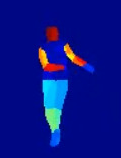
\includegraphics[width=0.3\linewidth]{sr-dense}
    \caption{Jumper wrapping the rope, denseposed}
    \label{proposal-fig:srwrapdense}
\end{figure}

Densepose seems to be able to give the bounding boxes of the main poses detected. Perhaps just a convex hull and some padding will be enough for smart cropping and training a network from scratch is not needed.
However, a local tryout (without boxes) was rather slow, 1.2 fps on GPU within a Docker container, on a laptop.
As jumpers don’t move that much most of the time, skipping some frames and smoothing out the prediction over the rest of the sequence or decreasing the amount of skipped frames when movement is detected, can speed up the localization.

Even when Densepose isn’t used, smoothing can still be applied to the guessed box as a video is basically a sequence of images.

\subsection{Video action segmentation}

When the athletes are cropped, videos need to be split\footnote{Not real/physical splits, but rather labels/annotations for where to split} in (sub)skills, because splitting new videos manually takes to much time and is impractical on competitions. A model like LTContext \textcite{Jiaming_2023} or others\footnote{Using sources like \href{https://paperswithcode.com/task/action-segmentation}{paperswithcode/action-segmentation}} would be appropriate.
Just like the localization, denseposing, extracting poses, foreground, background\dots would improve the segmentation.

The model for generating skill snapshots will
be useful for judging and subsequently labeling
data. Rather than replaying the video, judges can
just sequentially go through each trick one at a
time to assign, annotate or validate the predicted
skill.

\subsection{Skill recognition}
\label{proposal-subsec:skill-recognition}

The final step would be to recognize the total skill in a freestyle video.
\textcite{Yin_2024} did a general HAR survey, also focused on team sports in which they describe the evolution from normal CNN architectures, to recurrent neural networks for time sequences, remembering context, like the Long Short Term Memory model (LSTM). Then combining CNN output into LSTM or even implementing a convolutional filter in the memory cell \autocite{Shi_2015}.

\textcite{Wang_2019} investigated an improvement for current convolutional or recurrent models. They found that LSTM memory cells were too simple to contain higher-order complexities. As a result, they designed a memory in memory component, to replace the previous cell, which could predict actions on complexer data sets. This quickly formed the name Memory in Memory, MIM. Later, \textcite{Lin_2020} used a self-attention memory cell inside the convLSTM that can memorize global aspects in time and space. With about 35\% the number of parameters compared to Wang's MIM-model, SAM achieved a similar score as on the moving MNIST dataset, but faster. Although the focus of these papers was predicting future actions, the output can be transformed into a classification model, rather than a prediction model.

Another approach would be using transformers as a described possibility in \textcite{Yin_2024}, namely ViT-TAD model by \textcite{Yang_2023}, Swin transformer \textcite{Liu_2021} or VideoMAE v2 by \textcite{Wang_2023} seem good options, but further research/try-outs will be required to ensure the transfer models can predict actions.

For reference, NextJump uses a CNN - MobileNetv4, \autocite{MobileNetv4_2024} and a transformer to analyze the full sequence and count. So using the convLSTM, SAM, MobileNet, or a transformer brings us to a better definition or example of what exactly we want to predict.


\subsection{Skill-matrix - complexity \& levels - towards model accuracy}
\label{proposal-subsec:proposal-skillcomplexiteit}

\begin{figure}
    \centering
    \includegraphics[width=0.95\linewidth]{doubledutch-matrix}
    \caption[skill-matrix-DD]{Representation of a skill-matrix used for Doube Dutch}
    \label{proposal-fig:doubledutch-skill-matrix}
\end{figure}

A basic explanation of skills with some examples was given earlier. In order to recognize all skills, they should be worked out as good as possible. This section explains the composition of the skill-matrix, in order to give a better understanding on the total accuracy of the models later on. As described earlier, skills come with many transitions, take the first skill-matrix representation in figure \ref{proposal-fig:doubledutch-skill-matrix} to better understand skills and transitions.

\textbf{Type:} You have four styles of turning in double dutch; the normal way or double dutch (DD), reversing the rope rotation, sort of like backwards called irish dutch (irish), the chinese way of turning, chinese wheel (CW) or only using one rope or the two combined as a single rope, called single dutch or one rope.

\textbf{Rotations:} The amount of ropes passing underneath the athlete in one jump.

\textbf{Turner:} There are two turners, so two columns, where each turner can execute a turner involvement. Examples are EB, toad or crouger. The cross is in most cases performed by both turners, otherwise the ropes are tangled.

\textbf{Skills:} Mostly powers or gymnastics, but could also be footwork \footnote{Footwork will not be further specified in this paper}. Further distinction or organizing can happen as variation and transitions of powers and gymnastics exists. A recap of different skills would be: pushups, splits, crabs, frogs, swift, cartwheel, salto, webster, suicide, handsprings, round offs \dots % TODO : refer pictures, examples of skills in attachment.
Depending on the exact power or gymnastic, certain characteristics or transitions could be applied:

\begin{itemize}
    \item one handed
    \item one or two feet push-off (e.g. frog vs high frog, salto vs webster, suicide one vs two legged push-off)
    \item turntable \footnote{On way of turning your bodyposition, can be done per quarter e.g. quarter turntable push-up}
    \item full body rotation \footnote{Other way of turning your body, requires full turns}
    \item consecutive \footnote{Consecutive handstands are considered harder and thus get you extra points, not the case with push-up}, e.g. frog after frog
\end{itemize}

Applying these transitions, characteristics allows for more variation, which gets you more points. Repeated skills doesn't get you points. Repetitions are only defined by the skills in the ropes, the speed of the rope (rotations) and the type of turning \footnote{No difference will be made between irish turning and double dutch. Also, only the first skill in single dutch counts}.

\medskip

The skill-matrix is subject to change over time, initial skills not fitting the matrix will be left out for the MVP. Other than skills, jumpers and turners can switch with each other, most of these are also omitted in the MVP.
Each column in the skill-matrix-example 5 can only contain one answer, for which softmax can be used, while between multiple columns, no relation is required and can be predicted separately. This can be solved using a multi-branch output as described in by \autocite{Coulibaly_2022}). This can result in a guessed skill being partially correct, e.g. turner correct, but wrong rotational amount.

On another note, \textcite{Guo_2017} explain that softmax isn't always a good indicator of confidence. They mention that when a model has good calibration, the accuracy should align with the confidence of the prediction. E.g. when you predict a skill has 80\% chance being a push-up, then this prediction or 80\% of the predicted push-ups should be correct. Predictions using softmax tend to be overconfident.

\subsection{Group activity}

As DD3 is a group activity, problems could arise while trying to detect skills. However, the hypothesis is that a DD3 freestyle always acts as one unit, thus not really requiring much special attention. This could pose a problem when adapting SR to SR2 where two individuals are not exactly one unit. Some further research can be done in models like stagNet \autocite{Qi_2020} to improve, incorporate this idea.

\subsection{Unknown/Unusual skills}
\label{proposal-subsec:literature-unknown-unusual-skills}

Unknown skills or special cases pose a problem. That’s why the skill-matrix needs to defined
in such a way that new combinations can fit the matrix as much as possible and/or in combination with zero-shot learning. (Sort of marking unique skills as ’I don’t know’ so that others new/unique ones will also be marked as ’I don’t know’) Unusual skills on the other hand should be incorporated into the implementation.
Earlier an example was given about knocking 3 times on the door. A more concrete example would be turntables, which are mainly performed using a crab or push-up, but also seen with a frog or a split.
Turntables even have the potential to be combined with a swift. Omitting turntable frogs or splits in the train dataset can test this the ability to perform on unusual skills.

\subsection{Summary literature}
\label{proposal-subsec:summary literature}

The PoC needs to localize the jumper \footnote{which can use fine-tuned pre-trained models}, segment actions, and using labeled splits or guessed ones to predict (sub)skills.
Predicted skills will then be mapped to their corresponding level.

%---------- Methodology -------------------------------------------------------
\section{Methodology}%
\label{proposal-sec:methodoly}

After some more research about transformers and how to apply them for skill recognition and another non-transformer models besides convLSTM \& SAM to predict skills, the build process can start.
Using Canva, a \href{https://www.canva.com/design/DAGVz44QCgc/\_Mr9BrOqwwdy9cf-ieYFVg/edit?utm\_content=DAGVz44QCgc\&utm\_campaign=designshare\&utm\_medium=link2\&utm\_source=sharebutton}{user story map} is created to effectively see which tasks need to be done.

\subsection{General \& label location}

\begin{itemize}
    \item overview videos: navigate, filter, rename
    \item view video info, could have edit
    \item label inappropriate/blurry moments (idea: could be used, rather not)
    \item label passage/empty (livestream/wait) moments (idea: no skills)
    \item label jumper location
    \item Statistics of the general data distribution
\end{itemize}

\subsection{Predict location}

\begin{itemize}
    \item visualize jumpoer location predictions
    \item edit borders from new predictions
    \item visualize biggest localization mistakes (within video)
    \item visualize biggest localization mistakes (over all videos)
    \item localization model statistics
    \item data augmentation (if needed)
\end{itemize}

\subsection{Label action segments + label skills}

\begin{itemize}
    \item Label video action segment
    \item Loop-replay action segment
    \item Label segmented skills names
    \item mark false skills
    \item skills to level mapper (should have)
    \item search skills by name (could have)
    \item mark execution scale (could have)
    \item skilldistribution statistics (+/- distributionmatrix)
\end{itemize}

\subsection{Predict action segments}

\begin{itemize}
    \item visualize \& compare AI segmented skills
    \item visualize AI segmented skills from new videos (with confidence levels?)
\end{itemize}


\subsection{Predict skills}

\begin{itemize}
    \item model predicts levels (1-8 classes)
    \item model predicts variation element (4/6 classes)
    \item model predicts skill
    \item add judge scores to freestyles
    \item visualize \& compare AI labeled skills \& compare with total (judge)score
    \item validate AI recognized skills \& save as new training input
    \item label AI recognized skills as new or "i don't know"
    \item action segmentation stats
    \item skillrecognition stats
\end{itemize}


\subsection{Bis}

\begin{itemize}
    \item Language
    \item add competition jump order (easy recordings)
    \item stats competition
    \item insert multiple judge systems
\end{itemize}



\subsection{Answering sub-questions}
\label{proposal-subsec:methodology-sub-questions}



Most answers on the research (sub-)questions are woven into the literature, while others need to wait on the proof of concept to be fully answered.
While labeling skills an answer can be given to question \ref{proposal-subsubsec:proposal-intro-question-acceptable-results} acceptable results. The effective usage of models and architectures \ref{proposal-subsubsec:proposal-intro-question-earlier-research-guidance} and the educated guess about the data-amount needed to achieve better results \ref{proposal-subsubsec:proposal-intro-question-expected-data-to-increase-accuracy} will be answered soon


\subsection{Training \& Hardware}

Working with videos alone requires a lot of resources, let alone training on the data with a normal laptop. It is best to work with one or more GPUs to aid the research process. In between, calculations can be made to estimate how long training sessions will take. This also gives a future reference for other computer vision concepts.


%---------- Verwachte resultaten ----------------------------------------------
\section{Expected results}
\label{proposal-sec:verwachte-resultaten}

Localization of the jumper shouldn't pose an issue. It's would be safe to say that a quick progression towards video action segmentation can be made. Even if segmented actions do not overlap with their actual skills, it's not that hard of a block for the skill recognition part. It would just mean, that skillrecognition can not be applied on new unsegmented videos.
It's expected that SAM will prove to give better results than his base convLSTM model and a transformer probably even better if correctly integrated.

On the long run, it's expected to surpass judges in accuracy.

To answer the questions asked in the introduction a list of unknown or potential answers.

\begin{itemize}
    \item How will the model be built? --> unknown
    \item What would be the main structure of the model? --> unknown
    \item Which human activity recognition examples can be used or altered as the base of the model? --> aligns with modelselection
    \item When are AI-recognitions acceptable to potentially use on competitions? --> when they score equally as good as a judge and can flag or anticipate unknowns.
    \item How much data is expected to increase the accuracy off the Judge. --> we'll know later
    \item How can we use the AI-Judge to improve judges? --> correcting/assisting them.
    \item What needs to changed to a working model, to apply it on other judge-sports such as gymnastics, synchronized swimming... --> define a skill-matrix \& data
\end{itemize}


\section{Expected conclusion}%
\label{proposal-sec:conclusion}

The AI-Judge can improve fairness of judging on competitions by annotating skills and, when expanded, giving confidence levels to the skills it predicted. Using AI-Judge, more transparency towards scores can increase competitiveness or enable the public to better understand the scores. Even using the model to display snapshots of freestyles along the predicted skill and confidence score in total.

This AI-Judge can be extended towards other disciplines or different sports like acro, figure skating, gymnastics or dressage, to achieve similar results.

The next steps will be extending freestyle judging into DD4, SR2 and special skills.


%%---------- Andere bijlagen --------------------------------------------------
% TODO: Voeg hier eventuele andere bijlagen toe. Bv. als je deze BP voor de
% tweede keer indient, een overzicht van de verbeteringen t.o.v. het origineel.
%\input{...}
\chapter{\IfLanguageName{dutch}{Voorstelling van skills en draaierstrucs}{Display of skills and turners}}%
\label{ch:skills and turners}


In this appendix, skills will be displayed to give an example what exactly needs to be recognized. The focus of the first section is showing some subdisciplines of jump rope. The second part involves displaying performed skills and turners in Double Dutch.

\section{Jump Rope Disciplines}
\label{subsubsec:jump-rope-disciplines}

This section will focus on showing images of subdisciplines to make clear what entails each discipline.

\begin{figure}
    \centering
    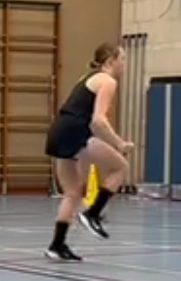
\includegraphics[width=0.32\linewidth]{img/sr-speed-c}
    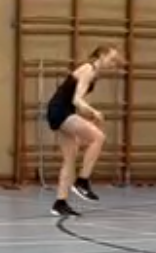
\includegraphics[width=0.32\linewidth]{img/sr-speed-le}
    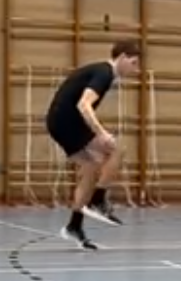
\includegraphics[width=0.32\linewidth]{img/sr-speed-m}
    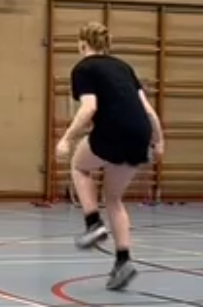
\includegraphics[width=0.4\linewidth]{img/sr-speed-lo}
    \label{fig:sr-speed-c}
    \caption[Jumpers performing single rope speed]{Jumpers performing single rope speed.}
\end{figure}

\begin{figure}
    \centering
    \includegraphics[width=0.4\linewidth]{img/sr.png}
    \caption[Athlete in a Single Rope routine]{Athlete in a Single Rope routine doing a wrap.}
    \label{fig:sr-wrap}
\end{figure}




\begin{figure}
    \centering
    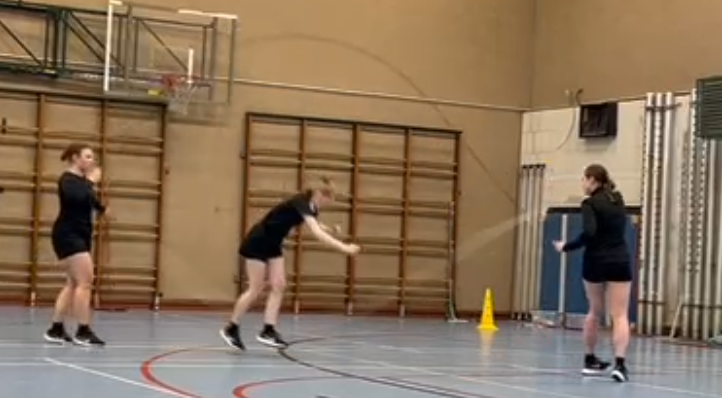
\includegraphics[height=0.14\linewidth]{img/dd3-du-flip-ts-1}
    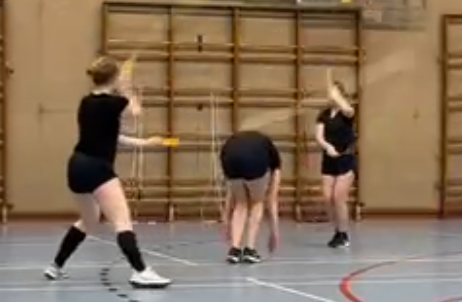
\includegraphics[height=0.14\linewidth]{img/dd3-du-crab-cross-1}
    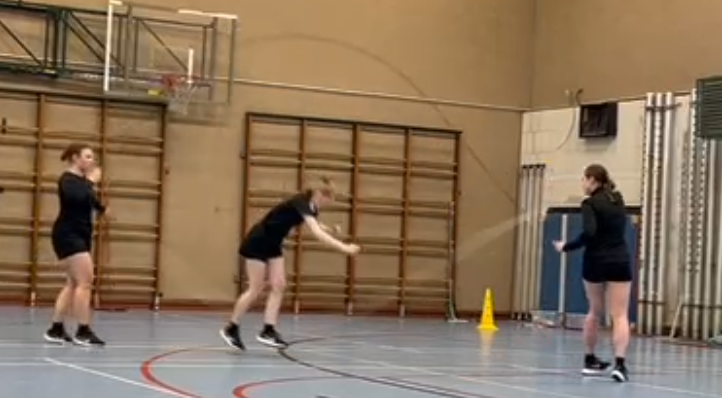
\includegraphics[height=0.14\linewidth]{img/dd3-du-flip-ts-1}
    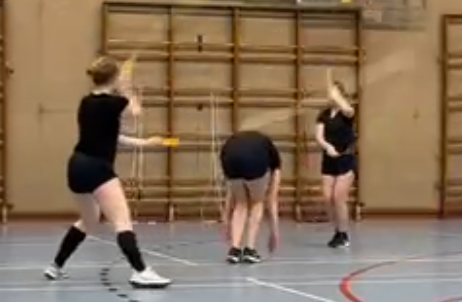
\includegraphics[height=0.14\linewidth]{img/dd3-du-crab-cross-1}
    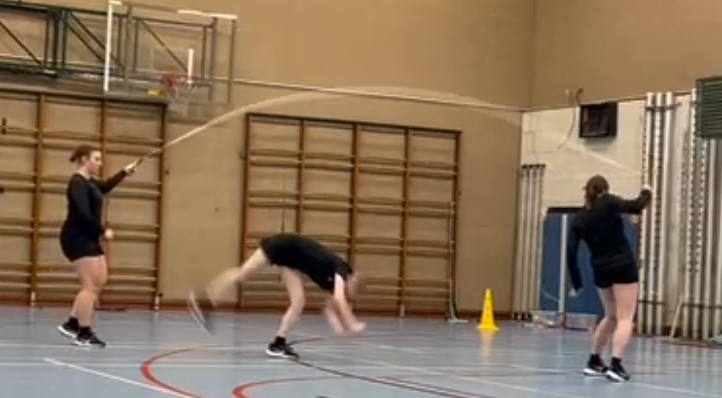
\includegraphics[height=0.14\linewidth]{img/dd3-du-flip-ts-2}
    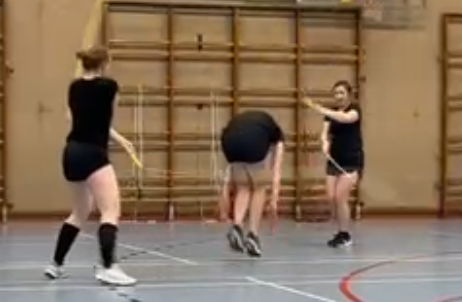
\includegraphics[height=0.14\linewidth]{img/dd3-du-crab-cross-2}
    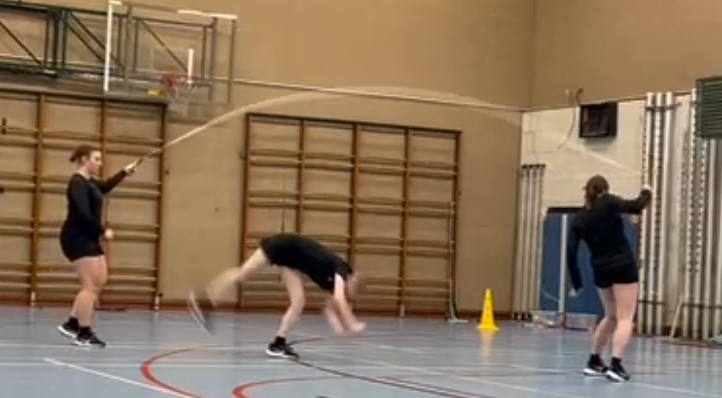
\includegraphics[height=0.14\linewidth]{img/dd3-du-flip-ts-2}
    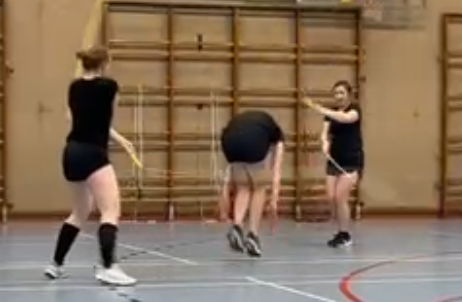
\includegraphics[height=0.14\linewidth]{img/dd3-du-crab-cross-2}
    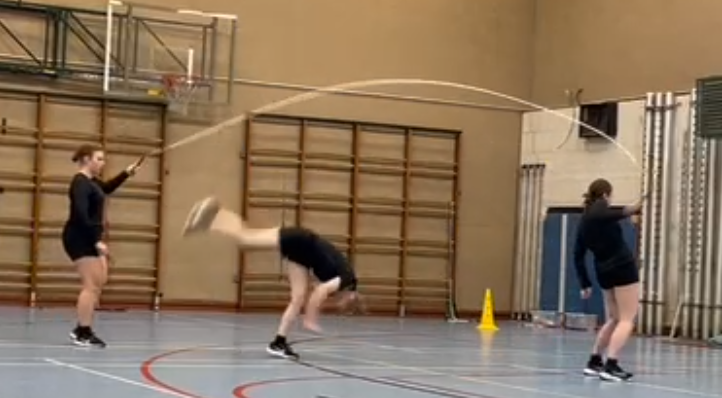
\includegraphics[height=0.14\linewidth]{img/dd3-du-flip-ts-3}
    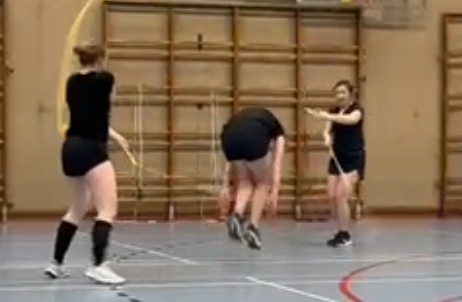
\includegraphics[height=0.14\linewidth]{img/dd3-du-crab-cross-3}
    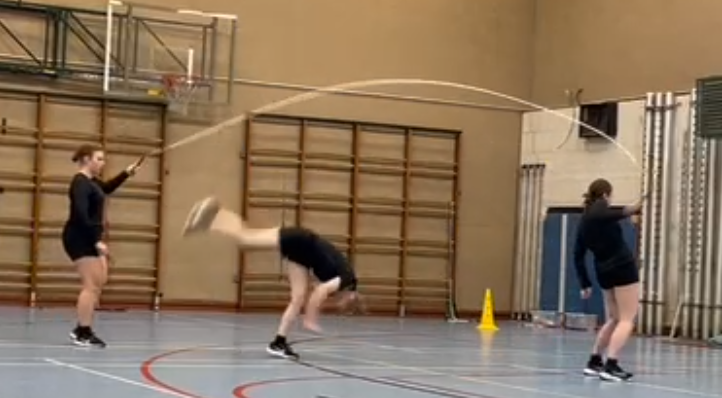
\includegraphics[height=0.14\linewidth]{img/dd3-du-flip-ts-3}
    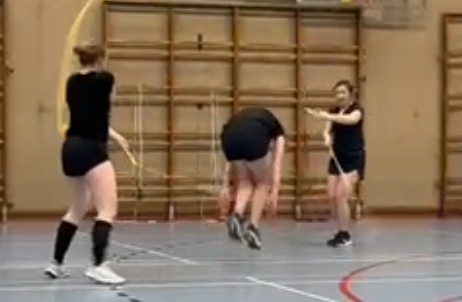
\includegraphics[height=0.14\linewidth]{img/dd3-du-crab-cross-3}
    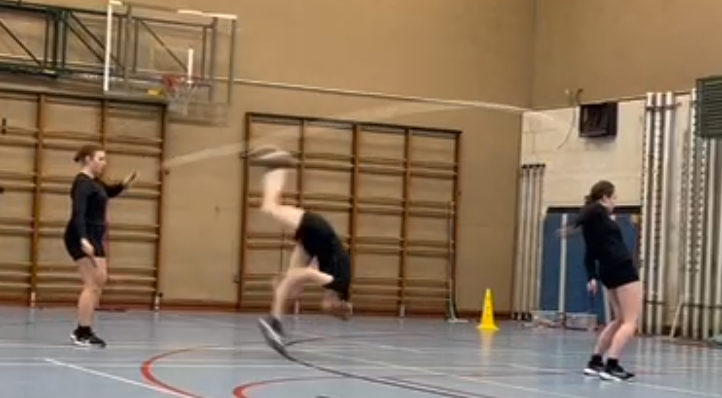
\includegraphics[height=0.14\linewidth]{img/dd3-du-flip-ts-4}
    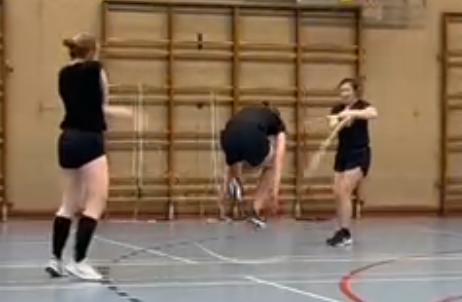
\includegraphics[height=0.14\linewidth]{img/dd3-du-crab-cross-4}
    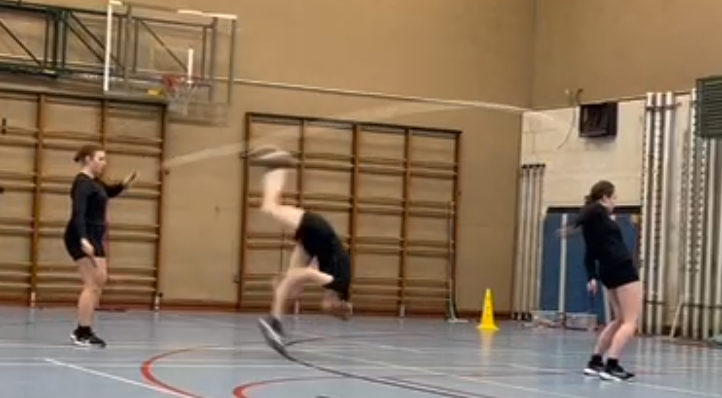
\includegraphics[height=0.14\linewidth]{img/dd3-du-flip-ts-4}
    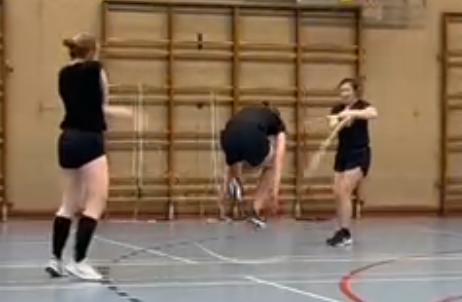
\includegraphics[height=0.14\linewidth]{img/dd3-du-crab-cross-4}
    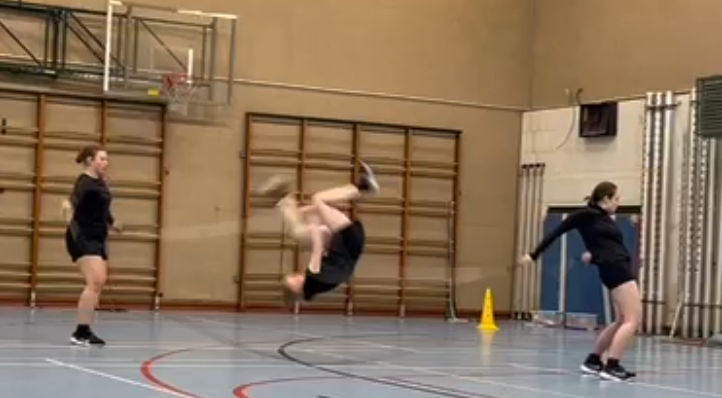
\includegraphics[height=0.14\linewidth]{img/dd3-du-flip-ts-5}
    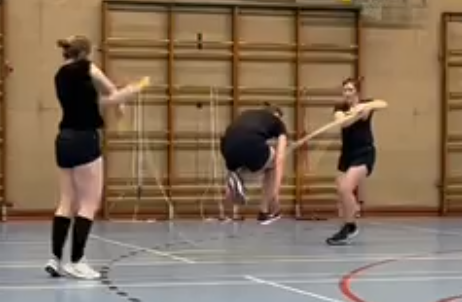
\includegraphics[height=0.14\linewidth]{img/dd3-du-crab-cross-5}
    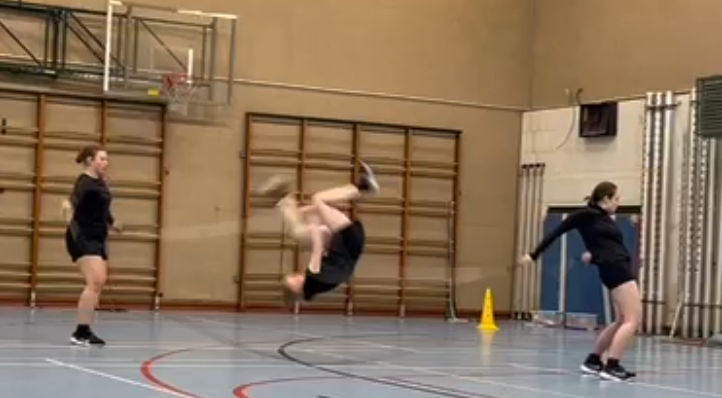
\includegraphics[height=0.14\linewidth]{img/dd3-du-flip-ts-5}
    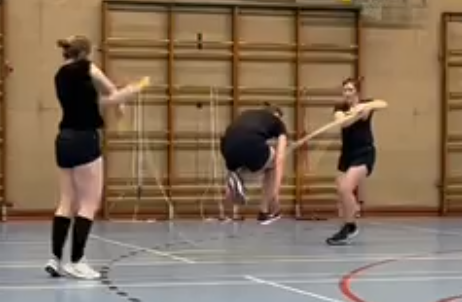
\includegraphics[height=0.14\linewidth]{img/dd3-du-crab-cross-5}
    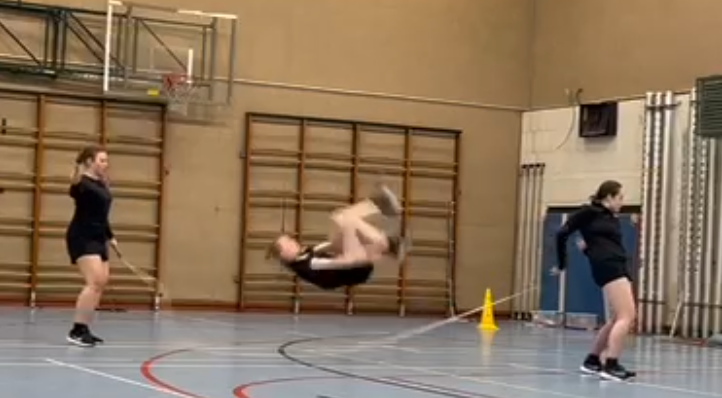
\includegraphics[height=0.14\linewidth]{img/dd3-du-flip-ts-6}
    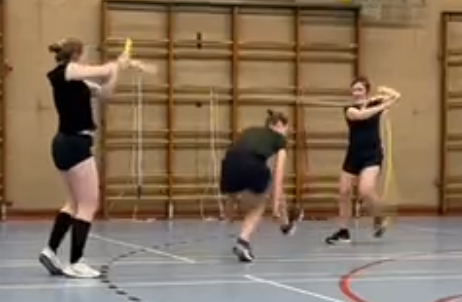
\includegraphics[height=0.14\linewidth]{img/dd3-du-crab-cross-6}
    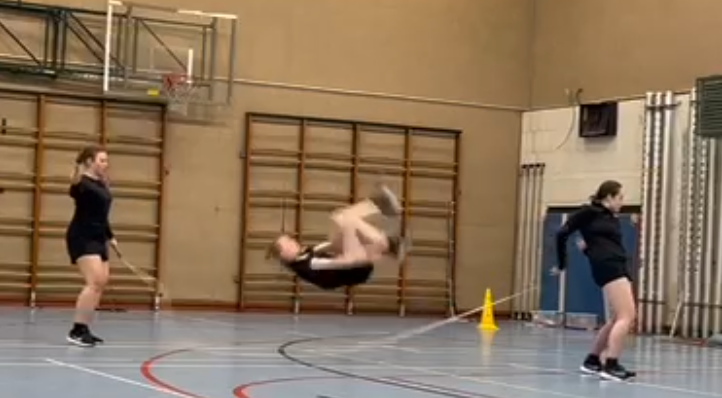
\includegraphics[height=0.14\linewidth]{img/dd3-du-flip-ts-6}
    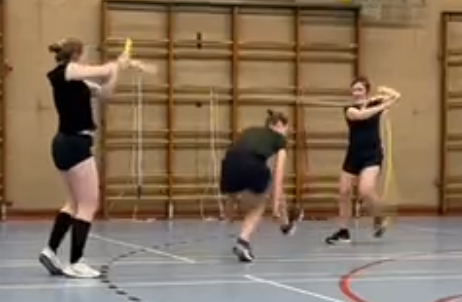
\includegraphics[height=0.14\linewidth]{img/dd3-du-crab-cross-6}
    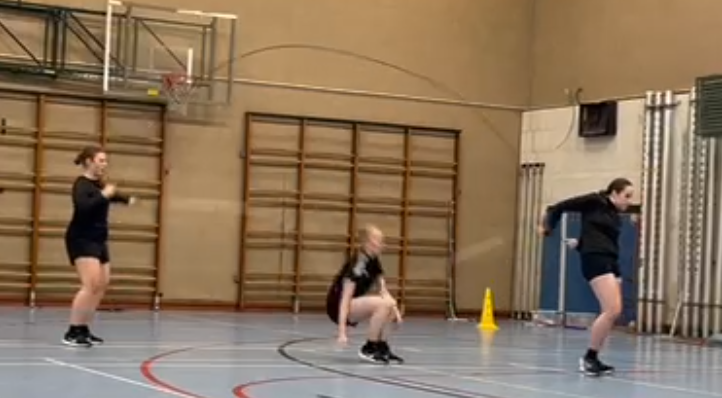
\includegraphics[height=0.14\linewidth]{img/dd3-du-flip-ts-7}
    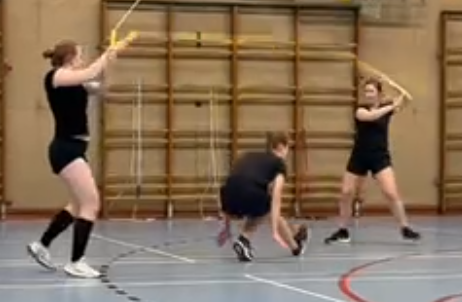
\includegraphics[height=0.14\linewidth]{img/dd3-du-crab-cross-7}
    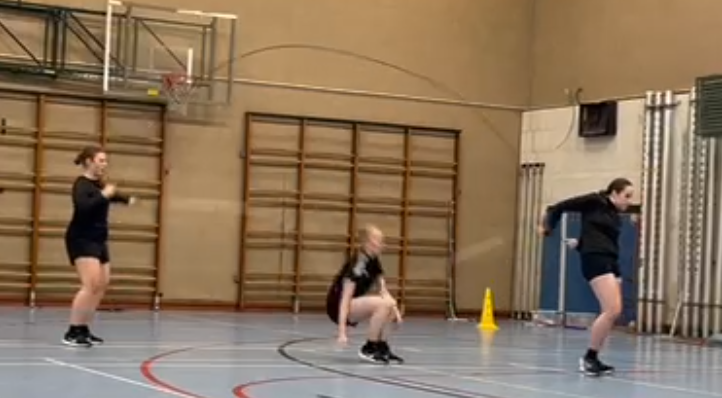
\includegraphics[height=0.14\linewidth]{img/dd3-du-flip-ts-7}
    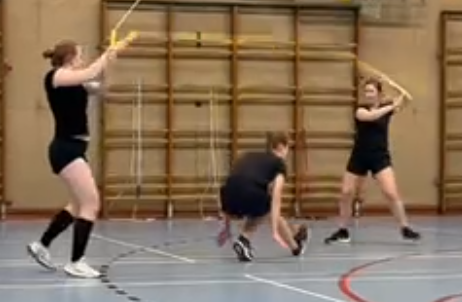
\includegraphics[height=0.14\linewidth]{img/dd3-du-crab-cross-7}
    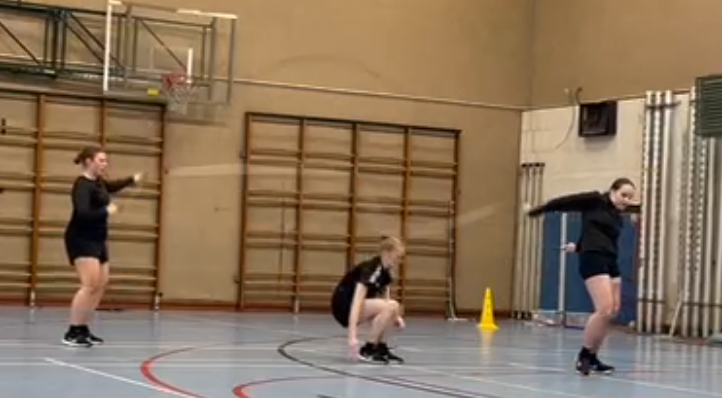
\includegraphics[height=0.14\linewidth]{img/dd3-du-flip-ts-8}
    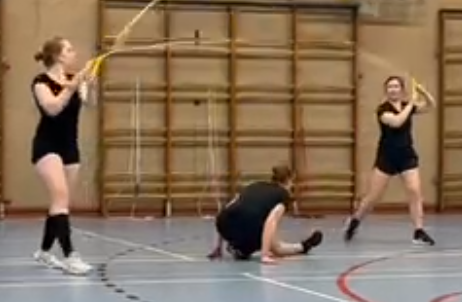
\includegraphics[height=0.14\linewidth]{img/dd3-du-crab-cross-8}
    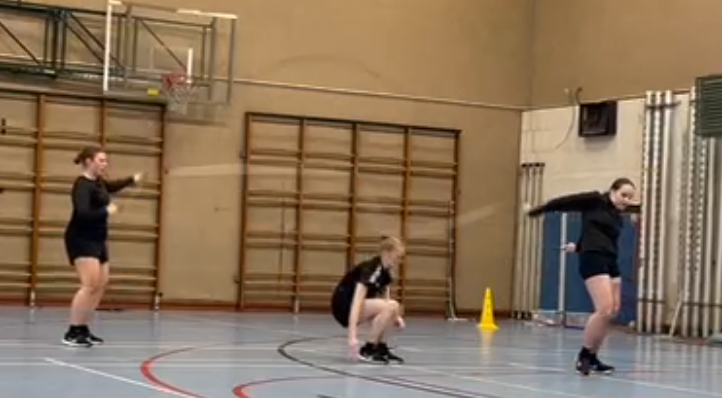
\includegraphics[height=0.14\linewidth]{img/dd3-du-flip-ts-8}
    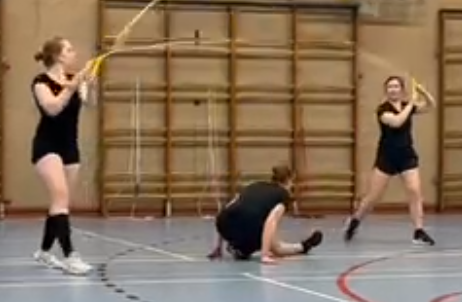
\includegraphics[height=0.14\linewidth]{img/dd3-du-crab-cross-8}
    \label{fig:skills}
    \caption[DD3 skill flows]{
        Display of 4 skills (currently only 2, 2 others will be added later) \\
        1: A flip while with double under and a TS restriction. \\
        2: A double under with two crosses, while the jumper lands in a crab position. \\
        3: Currently a duplicate of 1 \\
        4: Currently a duplicate of 2 \\
    }
\end{figure}
\chapter{\IfLanguageName{dutch}{Stukken code}{Code snippets}}%
\label{ch:code-snippets}


In this appendix, code snippets to prevent code saturation in between text.

(Code example will be deleted in the final submit)

\begin{listing}
    \begin{minted}{python}
        import pandas as pd
    \end{minted}
    \caption[]{}
    \label{code:}
\end{listing}


\section{Localization}
\label{sec:code-localization}

\begin{listing}
    \begin{minted}{python}
        DefaultMaxPool = functools.partial(
            keras.layers.MaxPool2D,
            pool_size=(3,3), strides=(2,2), padding="same")

        def get_googlenetsmall_model(input_shape, num_classes, use_batch_norm=True, **kwargs):
            model = keras.Sequential(**kwargs)
            model.add(keras.layers.Input(shape=input_shape))
            model.add(DefaultConv(filters=24, kernel_size=(7,7), strides=(2,2),  padding='same'))
            if use_batch_norm:
                model.add(keras.layers.BatchNormalization())
            model.add(DefaultMaxPool())
            model.add(DefaultConv(filters=32))
            model.add(DefaultConv(filters=48, kernel_size=(3,3)))
            if use_batch_norm:
                model.add(keras.layers.BatchNormalization())
            model.add(DefaultMaxPool())

            model.add(InceptionModule(filters11=32, filters33_reduce=48, filters33=64,
                filters55_reduce=8, filters55=16, filters_pool_proj=16,
                use_batch_norm=use_batch_norm))
            model.add(InceptionModule(filters11=64, filters33_reduce=64, filters33=96,
                filters55_reduce=16, filters55=48, filters_pool_proj=32,
                use_batch_norm=use_batch_norm))
            model.add(DefaultMaxPool())

            # ... see part 2
    \end{minted}
    \caption[GoogleNet implementation part 1]{GoogleNet implementation part 1}
    \label{code:keras-googlenet-small-replication}
\end{listing}

\begin{listing}
    \begin{minted}{python}
        def get_googlenetsmall_model(input_shape, num_classes, use_batch_norm=True, **kwargs):
            # ... see part 1

            model.add(InceptionModule(filters11=96, filters33_reduce=48, filters33=104,
                filters55_reduce=8, filters55=24, filters_pool_proj=32,
                use_batch_norm=use_batch_norm))
            model.add(InceptionModule(filters11=80, filters33_reduce=56, filters33=224,
                filters55_reduce=12, filters55=32, filters_pool_proj=32,
                use_batch_norm=use_batch_norm))
            model.add(InceptionModule(filters11=64, filters33_reduce=64, filters33=256,
                filters55_reduce=12, filters55=32, filters_pool_proj=32,
                use_batch_norm=use_batch_norm))
            model.add(InceptionModule(filters11=56, filters33_reduce=64, filters33=144,
                filters55_reduce=16, filters55=32, filters_pool_proj=32,
                use_batch_norm=use_batch_norm))
            model.add(InceptionModule(filters11=128, filters33_reduce=80, filters33=160,
                filters55_reduce=16, filters55=64, filters_pool_proj=64,
                use_batch_norm=use_batch_norm))

            model.add(DefaultMaxPool())
            model.add(InceptionModule(filters11=128, filters33_reduce=80, filters33=160,
                filters55_reduce=16, filters55=64, filters_pool_proj=64,
                use_batch_norm=use_batch_norm))
            model.add(InceptionModule(filters11=192, filters33_reduce=92, filters33=192,
                filters55_reduce=24, filters55=64, filters_pool_proj=64,
                use_batch_norm=use_batch_norm))
            model.add(keras.layers.GlobalAveragePooling2D())
            model.add(keras.layers.Dropout(0.4))
            model.add(keras.layers.Flatten())
            model.add(keras.layers.Dense(units=256, activation="relu"))
            model.add(keras.layers.Dense(units=num_classes, activation='sigmoid'))

            return model
    \end{minted}
    \caption[GoogleNet implementation part 1]{GoogleNet implementation part 2}
    \label{code:keras-googlenet-small-replication}
\end{listing}


\begin{listing}
    \begin{minted}{python}
        import functools
        import keras

        DefaultConv = functools.partial(
            keras.layers.Conv2D, kernel_size=(3, 3), strides=(2, 2),
            padding="same", activation="relu", kernel_initializer="he_normal")

        DefaultMaxPool = functools.partial(
            keras.layers.MaxPool2D,
            pool_size=(3,3), strides=(2,2), padding="same")

        def get_model(modelinfo: dict, **kwargs):
            dim = modelinfo['dim']
            model = keras.Sequential(**kwargs)
            mobilenetv3small = keras.applications.MobileNetV3Small(
                input_shape=(dim,dim,3),
                include_top=False,
                weights="imagenet",
                dropout_rate=0.2,
                pooling='avg',
                name="MobileNetV3Small",
            )
            mobilenetv3small.trainable = False
            model.add(mobilenetv3small)
            model.add(keras.layers.Dense(units=512, activation="relu"))
            model.add(keras.layers.Dense(units=128, activation="relu"))
            model.add(keras.layers.Dense(units=4, activation='sigmoid'))

            return model
    \end{minted}
    \caption[keras mobilenet full boxes]{Usage of mobilenet for full box predictions}
    \label{code:keras-mobilenetv3small}
\end{listing}

\begin{listing}
    \begin{minted}{python}
        # To long to properly include in the paper
        # https://github.com/mikeddecker/judge/blob/main/computervision/localizor_with_strats.py
    \end{minted}
    \caption[Localizor with strats]{Localizor with strats}
    \label{code:localizor-with-strats}
\end{listing}

\section{Segmentation}
\label{sec:code-segmentation}

\begin{listing}
    \begin{minted}{python}
        def calculate_splitpoint_values(videoId: int, frameLength:int, df_Skills:pd.DataFrame, fps:float, Nsec_frames_around=1/6):
        """Creates a dataframe: 'videoId', 'frameNr', 'splitpoint'
        Where splitpoint is the value 0 -> 1 whether the video needs to be split at that point or not"""
        splitpoint_values = {
            'videoId' : [videoId for _ in range(frameLength)],
            'frameNr' : range(frameLength),
            'splitpoint' : [0 for _ in range(frameLength)],
        }

        frames_around_splitpoint = round(Nsec_frames_around * fps)
        for _, skillrow in df_Skills.iterrows():
            frameStart = skillrow["frameStart"]
            frameEnd = skillrow["frameEnd"]

            currentFrameStart = frameStart - frames_around_splitpoint
            currentFrameEnd = frameEnd - frames_around_splitpoint
            while currentFrameStart < frameStart + frames_around_splitpoint:
                framesApart = abs(currentFrameStart - frameStart)
                splitvalue = 1 - (framesApart/frames_around_splitpoint) ** 2
                splitvalue *= splitvalue

                currentFrameStart += 1
                currentFrameEnd += 1

                splitpoint_values['splitpoint'][currentFrameStart] = splitvalue
                if currentFrameEnd < frameLength:
                    splitpoint_values['splitpoint'][currentFrameEnd] = splitvalue

        return pd.DataFrame(splitpoint_values)
    \end{minted}
    \caption[call-splitpoint-calculation]{call-splitpoint-calculation}
    \label{code:calculate-splitpoint-values}
\end{listing}


\begin{listing}
    \begin{minted}{python}
        df = calculate_splitpoint_values(
            videoId=videoId,
            frameLength=frameLength,
            df_Skills=self.Skills[self.Skills['videoId'] == videoId],
            fps = row["fps"]
        )
    \end{minted}
    \caption[call-splitpoint-calculation]{call-splitpoint-calculation}
    \label{code:call-splitpoint-calculation}
\end{listing}


\section{Recognition}
\label{sec:code-recognition}

\begin{listing}
    \begin{minted}{python}
        # ConfigHelper.py
        def get_discipline_DoubleDutch_config(include_tablename=True):
            config = {
                "Type" : ("Categorical", "Type"), # Will be textual representions
                "Rotations" : ("Numerical", 0, 8, 1), # min, max, step
                "Turner1": ("Categorical", "Turner"),
                "Turner2": ("Categorical", "Turner"),
                "Skill" : ("Categorical", "Skill"),
                "Hands" : ("Numerical", 0, 2, 1), # 0 for al salto types
                "Feet" : ("Numerical", 0, 2, 1),
                "Turntable" : ("Numerical", 0, 4, 0.25), # Per quarter (but still integers)
                "BodyRotations" : ("Numerical", 0, 2, 0.5),
                "Backwards" : ("Boolean"),
                "Sloppy" : ("Boolean"),
                "Hard2see" : ("Boolean"),
                "Fault" : ("Boolean"),
            }
            if include_tablename:
                config["Tablename"] = "DoubleDutch"
            return config
    \end{minted}
    \caption[confighelper skill configuration]{ConfigHelper skill configuration for labeling aspects of a skill, devided in Categorical, Numerical and Boolean output values of skills. All values of the numerical output are integers, which is why you need to multiply by the step in order to get the actual numerical representation.}
    \label{code:confighelper}
\end{listing}

\begin{listing}
    \begin{minted}{python}
        import keras
        import pandas as pd
        import tensorflow as tf
        import numpy as np
        import matplotlib.pyplot as plt
        import sys
        sys.path.append('..')
        from api.helpers import ConfigHelper
    \end{minted}
    \caption[imports-ViViT]{imports-ViViT}
    \label{code:imports-ViViT}
\end{listing}


\begin{listing}
    \begin{minted}{python}
        def mlp(x, hidden_units, dropout_rate):
            for units in hidden_units:
                x = keras.layers.Dense(units, activation=keras.activations.gelu)(x)
                x = keras.layers.Dropout(dropout_rate)(x)
            return x
    \end{minted}
    \caption[mlp layer]{ViViT: multi-layer-perceptron}
    \label{code:mlp-layer}
\end{listing}


\begin{listing}
    \begin{minted}{python}
    def __init__(self, patch_size):
        super().__init__()
        self.patch_size = patch_size

    def call(self, images):
        input_shape = keras.ops.shape(images)
        batch_size = input_shape[0]
        timestep = input_shape[1]
        height = input_shape[2]
        width = input_shape[3]
        channels = input_shape[4]
        num_patches_h = height // self.patch_size
        num_patches_w = width // self.patch_size

        def create_single_timepatch(video_input):
            patches = keras.ops.image.extract_patches(video_input, size=self.patch_size)
            patches = keras.ops.reshape(
                patches,
                (
                    num_patches_h * num_patches_w * timestep,
                    self.patch_size * self.patch_size * channels,
                ),
            )

            return patches

        patches = tf.map_fn(create_single_timepatch, images)

        return patches

    \end{minted}
    \caption[time-patches]{ViViT: Time Patches}
    \label{code:timepatches}
\end{listing}


\begin{listing}
    \begin{minted}{python}
        def get_model(modelinfo):
            inputs = keras.Input(shape = (modelinfo['timesteps'], modelinfo['dim'], modelinfo['dim'], 3))
            patches = TimePatches(modelinfo['patch_size'])(inputs)
            num_patches = (modelinfo['dim'] // modelinfo['patch_size']) ** 2
            encoded_patches = TimePatchEncoder(num_patches, modelinfo['timesteps'], modelinfo['dim_embedding'])(patches)
            print("shape of encoded_patches", encoded_patches.shape)

            # Create multiple layers of the Transformer block.
            for _ in range(modelinfo['encoder_blocks']):
                # Layer normalization 1.
                x1 = keras.layers.LayerNormalization(epsilon=1e-6)(encoded_patches)
                attention_output = keras.layers.MultiHeadAttention(
                num_heads=modelinfo['num_heads'], key_dim=modelinfo['dim_embedding'], dropout=0.1
                )(x1, x1)
                # Skip connection 1.
                x2 = keras.layers.Add()([attention_output, encoded_patches])
                # Layer normalization 2.
                x3 = keras.layers.LayerNormalization(epsilon=1e-6)(x2)
                x3 = mlp(x3, hidden_units=[modelinfo['dim_embedding'] ** 2, modelinfo['dim_embedding']], dropout_rate=0.1)
                # Skip connection 2.
                encoded_patches = keras.layers.Add()([x3, x2])

            # Create a [batch_size, projection_dim] tensor.
            representation = keras.layers.LayerNormalization(epsilon=1e-6)(encoded_patches)
            representation = keras.layers.Flatten()(representation)
            representation = keras.layers.Dropout(0.3)(representation)

            features = mlp(representation, hidden_units=modelinfo['mlp_head_units'], dropout_rate=0.3)

            ...

    \end{minted}
    \caption[get model ViViT]{ViViT: get model ViViT (keras), without output layer (part 1)
    (Possible bugfixes done using \textcite{OpenAI_ChatGPT_2025})}
    \label{code:get_model_ViViT}
\end{listing}

\begin{listing}
    \begin{minted}{python}
        # ... (this is the output layer of segmentation)
        classes = modelinfo['timesteps']
        outputs = keras.layers.Dense(classes, activation='softmax')(features)

        return keras.Model(inputs=inputs, outputs=outputs)
    \end{minted}
    \caption[ViViT output segmentation]{ViViT output segmentation using features of code fragment \ref{code:get_model_ViViT}}
    \label{code:ViViT-output-segmentation}
\end{listing}


\begin{listing}
    \begin{minted}{python}
        predictions = np.array(predictions)
        predictions_bigger_than_split_threshold = np.where(predictions > split_threshold, predictions, 0)
        p_split = predictions_bigger_than_split_threshold
        window_size = int(fps // 3)
        predictions_argMax_in_window = [s - window_size + np.argmax(p_split[max(0, s-window_size):min(frameLength, s+window_size)]) for s in range(frameLength)]
        predictions_splitmoments = np.where(predictions > split_threshold, predictions_argMax_in_window, 0)
        predictions_splitmoments = np.unique(predictions_splitmoments)

        distances = predictions_splitmoments[1:] - predictions_splitmoments[:-1]
        predictions_splitmoments = predictions_splitmoments[1:]
        predictions_splitmoments = predictions_splitmoments[np.where(distances < window_size // 3, False, True)]
        predictions_splitmoments = [int(g) for g in predictions_splitmoments]
    \end{minted}
    \caption[predictions-to-splitpoints]{Code which filters splitpoints from the raw predicted splitpoint values to frame numbers.}
    \label{code:predictions-to-splitpoints}
\end{listing}


\begin{listing}
    \begin{minted}{python}
        dd_config = ConfigHelper.get_discipline_DoubleDutch_config()
        outputs = {}
        for key, value in dd_config.items():
            if key == "Tablename":
                continue
            if value[0] == "Categorical":
                tablename = "skill"
                match (key):
                    case 'Skill':
                        tablename = 'skills'
                    case 'Turner1' | 'Turner2':
                        tablename = "turners"
                    case 'Type':
                        tablename = 'types'
                classes = int(df_table_counts.iloc[0][tablename] + 1) # Because of indexing
                outputs[key] = keras.layers.Dense(classes, activation='softmax', name=key)(features)
            else:
                outputs[key] = keras.layers.Dense(1, activation='sigmoid', name=key)(features)

        return keras.Model(inputs=inputs, outputs=outputs)
    \end{minted}
    \caption[Keras output layers for skills]{Keras output layers for skills}
    \label{code:keras-skill-top-layers}
\end{listing}

\begin{listing}
    \begin{minted}{python}
        def create_pytorch_skill_output_layers(lastNNeurons, balancedType, df_table_counts):
            dd_config = get_discipline_DoubleDutch_config()
            output_layers = torch.nn.ModuleDict()
            
            for key, value in dd_config.items():
                if key == "Tablename":
                    continue
                if value[0] == "Categorical":
                    columnname = "skill"
                    if key == 'Skill':
                        columnname = 'skills'
                    elif key in ['Turner1', 'Turner2']:
                        columnname = "turners"
                    elif key == 'Type':
                        columnname = 'types'
                    
                    classes = int(df_table_counts.iloc[0][columnname] + 1) # Because of MysqlIndex starts from 1
                    output_layers[key] = torch.nn.Linear(lastNNeurons, classes)
                else:
                    output_layers[key] = torch.nn.Linear(lastNNeurons, 1)
            
            if balancedType == 'jump_return_push_frog_other':
                output_layers['Skill'] = torch.nn.Linear(lastNNeurons, 5)
            
            return output_layers
    \end{minted}
    \caption[Pytorch skill output layers]{PyTorch skill output layers, uses \ref{code:confighelper}}
    \label{code:pytorch-skill-output-layers}
\end{listing}

\begin{listing}
    \begin{minted}{python}
        class MViT(nn.Module):
            def __init__(self, skill_or_segment:str, modelinfo:dict, df_table_counts:pd.DataFrame):
                super(MViT, self).__init__()
                self.modelinfo = modelinfo
                self.df_table_counts = df_table_counts
                self.isSkillModel = skill_or_segment == "skills"
                
                input_shape = (3, modelinfo['timesteps'], modelinfo['dim'], modelinfo['dim'])
                self.mvit = models.video.mvit_v1_b(weights='DEFAULT')
                self.mvit = self.mvit.to('cuda').eval()

                for param in self.mvit.parameters():
                    param.requires_grad = False

                self.mvit.head = torch.nn.Identity()  # This removes the top layer
                self.flatten = nn.Flatten()
                self.LastNNeurons = self._get_mvit_output(input_shape)
                
                if self.isSkillModel:
                    self.output_layers = create_pytorch_skill_output_layers(lastNNeurons=self.LastNNeurons, balancedType=modelinfo['balancedType'], df_table_counts = self.df_table_counts)
                else:
                    self.output_layer = create_pytorch_segmentation_output_layers(lastNNeurons=self.LastNNeurons, timesteps=modelinfo['timesteps'])

                
            def _get_mvit_output(self, shape):
                with torch.no_grad():
                    input = torch.rand(1, *shape).to('cuda')
                    output = self.mvit(input)
                    output = self.flatten(output)
                    return output.shape[1]
    \end{minted}
    \caption[Pytorch MViT implementation init]{Pytorch MViT implementation init, uses \ref{code:pytorch-skill-output-layers} and \ref{code:pytorch-skill-forward}}
    \label{code:pytorch-mvit-init}
\end{listing}

\begin{listing}
    \begin{minted}{python}
    def forward(self, x):
        # Input shape: (batch_size, channels, timesteps, height, width)
        x = self.mvit(x)
        x = self.flatten(x)
        
        if self.isSkillModel:
            return forward_skill_output_layers(features=x, output_layers=self.output_layers)
        else:
            return forward_segmentation_output_layers(features=x, output_layer=self.output_layer)
    \end{minted}
    \caption[Pytorch MViT forward]{Pytorch MViT implementation of forward method, used by \ref{code:pytorch-mvit-init}}
    \label{code:pytorch-skill-forward}
\end{listing}



\begin{listing}
    \begin{minted}{python}
        def forward_skill_output_layers(features: torch.tensor, output_layers: dict[str, torch.nn.Module]):
            outputs = {}
            for key, layer in output_layers.items():
                if key in ['Skill', 'Turner1', 'Turner2', 'Type']:
                    outputs[key] = layer(features)
                else:  # Regression outputs
                    outputs[key] = torch.sigmoid(layer(features))
            
            return outputs
    \end{minted}
    \caption[Pytorch skill forward feed]{PyTorch skill forward feeding}
    \label{code:pytorch-skill-layers-forward}
\end{listing}

\begin{listing}
    \begin{minted}{python}
        # Adapting the losses, as limiting to 10% can change occurences of faults, bodyrotations... a little
        for key, value in config.items():
            value_counts_train = train_generator.BalancedSet[ConfigHelper.lowerProperty(key)].value_counts(dropna=False)
            value_counts_val = val_generator.Skills[ConfigHelper.lowerProperty(key)].value_counts(dropna=False)
            value_counts_combined = value_counts_train.add(value_counts_val, fill_value=0)
        
            maximum = value_counts_combined.max()
        
            weights = (maximum + maximum // 8 - value_counts_combined).pow(0.75)
            weights = weights / weights.mean()
            if value[0] == 'Categorical':
                weights.loc[0] = 0
            weights = weights.sort_index()
        
            w_all = torch.ones(value_counts_combined.index.max() + 1, dtype=torch.float32).to(device=device)
            for idx, w in weights.items():
                w_all[idx] = w
            w_all = (w_all + 1) ** 2
        
            print("loss weights for", key, w_all)
            if value[0] == 'Categorical':
                loss_fns[key] = torch.nn.CrossEntropyLoss(w_all).to(device=device)
            else:
                loss_fns[key] = lambda input, target: weighted_mse_loss(input=input, target=target, weight=w_all)
    \end{minted}
    \caption[Code calculating weights for the loss functions]{Code calculating weights for the loss functions}
    \label{code:recognition-weighted-loss}
\end{listing}

\begin{listing}
    \begin{minted}{python}
        def weighted_mse_loss(input, target, weight):
            "https://discuss.pytorch.org/t/how-to-implement-weighted-mean-square-error/2547"
            return torch.sum(weight * (input - target) ** 2)
    \end{minted}
    \caption[Weihted MSE]{Weighted MSE}
    \label{code:weighted-mse}
\end{listing}



\chapter{\IfLanguageName{dutch}{Tabellen}{Tables}}%
\label{ch:tables}


\section{MViT classification result before weighted loss}

\begin{table}[h!]
    \begin{tabular}{|l|r|r|r|r|}
        \hline          & precision & recall & f1-score & support \\
        \hline
        Double Dutch    &   0.97    &   0.98    &   0.97    &  525 \\
        Single Dutch    &   1.00    &   0.25    &   0.40    &  4   \\
        Irish Dutch     &   0.00    &   0.00    &   0.00    &  0   \\
        Chinese Wheel   &   0.92    &   0.97    &   0.94    &  86  \\
        Transition      &   0.72    &   0.88    &   0.79    &  24  \\
        Snapperlike     &   0.90    &   0.63    &   0.75    &  30  \\
        \hline
        accuracy        &           &           &   0.95    &  669 \\
        macro avg       &   0.75    &   0.62    &   0.64    &  669 \\
        weighted avg    &   0.95    &   0.95    &   0.95    &  669 \\ \hline
    \end{tabular}
    \caption[Type distribution]{First MViT class report for type}
    \label{tbl:mvit-first-class-reports-type}
\end{table}

\begin{table}[h!]
    \begin{tabular}{|l|r|r|r|r|}
        \hline
          &  precision &   recall & f1-score &  support \\ \hline
        0 &       0.00 &     0.00 &     0.00 &       26 \\
        1 &       0.91 &     0.95 &     0.93 &      544 \\
        2 &       0.59 &     0.67 &     0.63 &       70 \\
        3 &       0.39 &     0.44 &     0.41 &       16 \\
        4 &       0.50 &     0.10 &     0.17 &       10 \\
        5 &       0.00 &     0.00 &     0.00 &        2 \\
        8 &       0.00 &     0.00 &     0.00 &        1 \\
        \hline
        accuracy &            &          &     0.86 &      669 \\
        macro avg &       0.34 &     0.31 &     0.31 &      669 \\
        weighted avg &       0.82 &     0.86 &     0.83 &      669 \\ \hline
    \end{tabular}
    \caption[Rotation distribution]{First MViT class report for rotations}
    \label{tbl:mvit-first-class-reports-rotations}
\end{table}

\begin{table}[h!]
    \begin{tabular}{|l|r|r|r|r|}
                \hline & precision &   recall & f1-score &  support \\ \hline
               normal &      0.93 &     0.98 &     0.96 &      542 \\
              crouger &      0.90 &     0.88 &     0.89 &       40 \\
                cross &      0.80 &     0.58 &     0.67 &       57 \\
             cross BW &      0.00 &     0.00 &     0.00 &        2 \\
   jump over cross BW &      0.00 &     0.00 &     0.00 &        3 \\
                   EB &      0.57 &     0.36 &     0.44 &       11 \\
                 toad &      0.54 &     0.88 &     0.67 &        8 \\
              toad BW &      0.00 &     0.00 &     0.00 &        1 \\
              EB toad &      0.00 &     0.00 &     0.00 &        3 \\
                   TS &      0.00 &     0.00 &     0.00 &        0 \\
         inverse toad &      0.00 &     0.00 &     0.00 &        0 \\
             elephant &      0.00 &     0.00 &     0.00 &        0 \\
         crougercross &      0.00 &     0.00 &     0.00 &        0 \\
             pinwheel &      0.00 &     0.00 &     0.00 &        1 \\
              suicide &      0.00 &     0.00 &     0.00 &        0 \\
      inverse crouger &      0.00 &     0.00 &     0.00 &        0 \\
                 flip &      0.00 &     0.00 &     0.00 &        0 \\
               T-toad &      0.00 &     0.00 &     0.00 &        0 \\
MULTIPLE TURNERSKILLS &      0.00 &     0.00 &     0.00 &        0 \\
           EB toad BW &      0.00 &     0.00 &     0.00 &        0 \\
         L2-power-gym &      0.00 &     0.00 &     0.00 &        0 \\
         L3-power-gym &      0.00 &     0.00 &     0.00 &        0 \\
         L4-power-gym &      0.00 &     0.00 &     0.00 &        0 \\
              UNKNOWN &      0.00 &     0.00 &     0.00 &        0 \\
         jump-through &      0.00 &     0.00 &     0.00 &        0 \\
      EB inverse toad &      0.00 &     0.00 &     0.00 &        1 \\ \hline
             accuracy &           &          &     0.91 &      669 \\
            macro avg &      0.14 &     0.14 &     0.14 &      669 \\
         weighted avg &      0.89 &     0.91 &     0.90 &      669 \\
         \hline
    \end{tabular}
    \caption[Turner 1 class report]{First MViT class report for turner1}
    \label{tbl:mvit-first-class-reports-turner1}
\end{table}

\begin{table}[h!]
    \begin{tabular}{|l|r|r|r|r|}
                \hline & precision &   recall & f1-score &  support \\ \hline
                normal &       0.92 &     0.97 &     0.94 &      540 \\
               crouger &       0.80 &     0.84 &     0.82 &       38 \\
                 cross &       0.79 &     0.60 &     0.68 &       55 \\
              cross BW &       0.00 &     0.00 &     0.00 &        4 \\
    jump over cross BW &       0.00 &     0.00 &     0.00 &        2 \\
                    EB &       0.67 &     0.31 &     0.42 &       13 \\
                  toad &       0.50 &     0.86 &     0.63 &        7 \\
               toad BW &       0.00 &     0.00 &     0.00 &        2 \\
               EB toad &       0.00 &     0.00 &     0.00 &        4 \\
                    TS &       0.00 &     0.00 &     0.00 &        0 \\
          inverse toad &       0.00 &     0.00 &     0.00 &        0 \\
              elephant &       0.00 &     0.00 &     0.00 &        0 \\
          crougercross &       0.00 &     0.00 &     0.00 &        0 \\
              pinwheel &       0.00 &     0.00 &     0.00 &        3 \\
               suicide &       0.00 &     0.00 &     0.00 &        0 \\
       inverse crouger &       0.00 &     0.00 &     0.00 &        0 \\
                  flip &       0.00 &     0.00 &     0.00 &        0 \\
                T-toad &       0.00 &     0.00 &     0.00 &        0 \\
 MULTIPLE TURNERSKILLS &       0.00 &     0.00 &     0.00 &        0 \\
            EB toad BW &       0.00 &     0.00 &     0.00 &        0 \\
          L2-power-gym &       0.00 &     0.00 &     0.00 &        0 \\
          L3-power-gym &       0.00 &     0.00 &     0.00 &        0 \\
          L4-power-gym &       0.00 &     0.00 &     0.00 &        0 \\
               UNKNOWN &       0.00 &     0.00 &     0.00 &        0 \\
          jump-through &       0.00 &     0.00 &     0.00 &        0 \\
       EB inverse toad &       0.00 &     0.00 &     0.00 &        1 \\ \hline
              accuracy &            &          &     0.90 &      669 \\
             macro avg &       0.14 &     0.14 &     0.13 &      669 \\
          weighted avg &       0.87 &     0.90 &     0.88 &      669 \\
         \hline
    \end{tabular}
    \caption[Turner 2 class report]{First MViT class report for turner2}
    \label{tbl:mvit-first-class-reports-turner2}
\end{table}

\begin{table}[h!]
    \begin{tabular}{|l|r|r|r|r|}
                \hline & precision &   recall & f1-score &  support \\ \hline
                jump &      1.00 &     0.98 &     0.99 &      380 \\
   return from power &      0.88 &     0.87 &     0.88 &       85 \\
              pushup &      0.84 &     0.96 &     0.90 &       72 \\
                frog &      0.96 &     0.90 &     0.93 &       61 \\
               split &      0.94 &     1.00 &     0.97 &       15 \\
             SPAGAAT &      0.00 &     0.00 &     0.00 &        0 \\
                crab &      0.64 &     0.88 &     0.74 &        8 \\
               swift &      0.00 &     0.00 &     0.00 &        0 \\
     mountainclimber &      0.00 &     0.00 &     0.00 &        0 \\
                 rad &      0.00 &     0.00 &     0.00 &        2 \\
              rondat &      0.40 &     0.40 &     0.40 &        5 \\
          handspring &      0.43 &     0.60 &     0.50 &        5 \\
                 kip &      1.00 &     0.83 &     0.91 &        6 \\
              kopkip &      0.50 &     1.00 &     0.67 &        1 \\
                flip &      0.50 &     0.60 &     0.55 &        5 \\
             arabian &      0.00 &     0.00 &     0.00 &        0 \\
             rol2kip &      0.83 &     0.83 &     0.83 &        6 \\
                roll &      1.00 &     0.67 &     0.80 &        3 \\
            leapfrog &      0.00 &     0.00 &     0.00 &        0 \\
             suicide &      0.89 &     0.89 &     0.89 &        9 \\
      flip-to-pushup &      0.00 &     0.00 &     0.00 &        1 \\
        buddy-bounce &      0.00 &     0.00 &     0.00 &        1 \\
                stut &      1.00 &     1.00 &     1.00 &        2 \\
       footwork-kick &      0.00 &     0.00 &     0.00 &        0 \\
               speed &      0.00 &     0.00 &     0.00 &        0 \\
       footwork-open &      0.00 &     0.00 &     0.00 &        1 \\
       footwork-knee &      0.00 &     0.00 &     0.00 &        0 \\
     footwork-cancan &      0.00 &     0.00 &     0.00 &        0 \\
      footwork-cross &      0.00 &     0.00 &     0.00 &        0 \\
              UNKOWN &      0.00 &     0.00 &     0.00 &        1 \\
        \hline
            accuracy &           &          &     0.93 &      669 \\
           macro avg &      0.39 &     0.41 &     0.40 &      669 \\
        weighted avg &      0.93 &     0.93 &     0.93 &      669 \\
         \hline
    \end{tabular}
    \caption[Skill class report]{First MViT class report for skill}
    \label{tbl:mvit-first-class-reports-skill}
\end{table}

\begin{table}[h!]
    \begin{tabular}{|l|r|r|r|r|}
                \hline & precision &   recall & f1-score &  support \\ \hline
                0 &      0.99 &     0.94 &     0.96 &      481 \\
                1 &      0.27 &     0.27 &     0.27 &       45 \\
                2 &      0.75 &     0.88 &     0.81 &      143 \\ \hline
         accuracy &           &          &     0.88 &      669 \\
        macro avg &      0.67 &     0.70 &     0.68 &      669 \\
     weighted avg &      0.89 &     0.88 &     0.88 &      669 \\
         \hline
    \end{tabular}
    \caption[Hands class report]{First MViT class report for hands}
    \label{tbl:mvit-first-class-reports-hands}
\end{table}

\begin{table}[h!]
    \begin{tabular}{|l|r|r|r|r|}
                \hline & precision &   recall & f1-score &  support \\ \hline
                0 &      0.94 &      0.70 &      0.80 &        67 \\
                1 &      0.52 &      0.52 &      0.52 &        83 \\
                2 &      0.92 &      0.95 &      0.94 &       519 \\
         accuracy &           &           &      0.87 &       669 \\ \hline
        macro avg &      0.80 &      0.72 &      0.75 &       669 \\
     weighted avg &      0.87 &      0.87 &      0.87 &       669 \\
         \hline
    \end{tabular}
    \caption[Feet class report]{First MViT class report for feet}
    \label{tbl:mvit-first-class-reports-feet}
\end{table}

\begin{table}[h!]
    \begin{tabular}{|l|r|r|r|r|}
                \hline & precision &   recall & f1-score &  support \\ \hline
                0 &      0.98 &     0.99 &     0.99 &      656 \\
                1 &      0.17 &     0.09 &     0.12 &       11 \\
                2 &      0.00 &     0.00 &     0.00 &        2 \\ \hline
         accuracy &           &          &     0.97 &      669 \\
        macro avg &      0.38 &     0.36 &     0.37 &      669 \\
     weighted avg &      0.97 &     0.97 &     0.97 &      669 \\
         \hline
    \end{tabular}
    \caption[Turntable class report]{First MViT class report for turntable}
    \label{tbl:mvit-first-class-reports-turntable}
\end{table}

\begin{table}[h!]
    \begin{tabular}{|l|r|r|r|r|}
                \hline & precision &   recall & f1-score &  support \\ \hline
                0 &      1.00 &      1.00 &     1.00 &      666 \\
                1 &      0.00 &      0.00 &     0.00 &        2 \\
                2 &      0.00 &      0.00 &     0.00 &        1 \\ \hline
         accuracy &           &           &     1.00 &      669 \\
        macro avg &      0.33 &      0.33 &     0.33 &      669 \\
     weighted avg &      0.99 &      1.00 &     0.99 &      669 \\

         \hline
    \end{tabular}
    \caption[Body rotations class report]{First MViT class report for bodyRotations}
    \label{tbl:mvit-first-class-reports-bodyRotations}
\end{table}

\begin{table}[h!]
    \begin{tabular}{|l|r|r|r|r|}
                \hline & precision &   recall & f1-score &  support \\ \hline
                0 &       0.99 &     1.00 &     1.00 &      660 \\
                1 &       0.80 &     0.44 &     0.57 &        9 \\ \hline
         accuracy &            &          &     0.99 &      669 \\
        macro avg &       0.90 &     0.72 &     0.78 &      669 \\
     weighted avg &       0.99 &     0.99 &     0.99 &      669 \\
         \hline
    \end{tabular}
    \caption[Backwards class report]{First MViT class report for backwards}
    \label{tbl:mvit-first-class-reports-backwards}
\end{table}

\begin{table}[h!]
    \begin{tabular}{|l|r|r|r|r|}
                \hline & precision &   recall & f1-score &  support \\ \hline
                0 &      0.97 &     1.00 &     0.99 &      651 \\
                1 &      0.00 &     0.00 &     0.00 &       18 \\
         accuracy &           &          &     0.97 &      669 \\ \hline
        macro avg &      0.49 &     0.50 &     0.49 &      669 \\
     weighted avg &      0.95 &     0.97 &     0.96 &      669 \\
         \hline
    \end{tabular}
    \caption[Sloppy class report]{First MViT class report for sloppy}
    \label{tbl:mvit-first-class-reports-sloppy}
\end{table}

\begin{table}[h!]
    \begin{tabular}{|l|r|r|r|r|}
                \hline & precision &   recall & f1-score &  support \\ \hline
                0 &      1.00 &     1.00 &     1.00 &      666 \\
                1 &      0.00 &     0.00 &     0.00 &        3 \\ \hline
         accuracy &           &          &     1.00 &      669 \\
        macro avg &      0.50 &     0.50 &     0.50 &      669 \\
     weighted avg &      0.99 &     1.00 &     0.99 &      669 \\

         \hline
    \end{tabular}
    \caption[Hard to see class report]{First MViT class report for hard2see}
    \label{tbl:mvit-first-class-reports-hard2see}
\end{table}

\begin{table}[h!]
    \begin{tabular}{|l|r|r|r|r|}
                \hline & precision &   recall & f1-score &  support \\ \hline
                0 &      0.96 &     1.00 &      0.98 &       639 \\
                1 &      0.00 &     0.00 &      0.00 &        30 \\ \hline
         accuracy &           &          &      0.96 &       669 \\
        macro avg &      0.48 &     0.50 &      0.49 &       669 \\
     weighted avg &      0.91 &     0.96 &      0.93 &       669 \\
         \hline
    \end{tabular}
    \caption[Fault class report]{First MViT class report for fault}
    \label{tbl:mvit-first-class-reports-fault}
\end{table}



%%---------- Backmatter, referentielijst ---------------------------------------

\backmatter{}

\setlength\bibitemsep{2pt} %% Add Some space between the bibliograpy entries
\printbibliography[heading=bibintoc]

\end{document}
